\section{System design} \label{sec:system_design}
In order to meet the requirements mentioned in the introduction, a topology of the voice communication system as shown in the figure \ref{fig:tikz_system_topology} was chosen. Voice communication takes place via the frequency $f_\sim = 158,950\mathrm{MHz}$ and the system consists of a \emph{base station} (BSt) -- which the OeWF refers to as \emph{operations} (OPS) -- an \emph{on-site support} (OSS) crew with handheld radios, a self-sufficient voice communication repeater -- which from now on will simply be refered to as \emph{repeater} (REP) -- \emph{analog astronauts} (AAs) using the \emph{Serenity} (SER) spacesuit simulator and the safety officers for the AAs. The latter also carry handheld radios.
\begin{figure}[h!]
	\centering
	

\tikzset{every picture/.style={line width=0.75pt}} %set default line width to 0.75pt        

\begin{tikzpicture}[x=0.75pt,y=0.75pt,yscale=-1,xscale=1]
%uncomment if require: \path (0,1074); %set diagram left start at 0, and has height of 1074

%Straight Lines [id:da776044312069671] 
\draw [color={rgb, 255:red, 155; green, 155; blue, 155 }  ,draw opacity=1 ]   (186.78,292.25) -- (186.81,286.3) ;
%Straight Lines [id:da8862888077148174] 
\draw [color={rgb, 255:red, 155; green, 155; blue, 155 }  ,draw opacity=1 ]   (181.51,294.03) -- (192.06,290.48) ;
%Shape: Rectangle [id:dp48061826630378013] 
\draw  [color={rgb, 255:red, 0; green, 41; blue, 90 }  ,draw opacity=1 ][fill={rgb, 255:red, 57; green, 107; blue, 163 }  ,fill opacity=1 ][line width=0.75]  (163.1,277.18) -- (188.58,283.72) -- (181.51,294.03) -- (156.02,287.48) -- cycle ;
%Straight Lines [id:da17291607219553407] 
\draw [color={rgb, 255:red, 0; green, 41; blue, 90 }  ,draw opacity=1 ][line width=0.75]    (162.21,278.47) -- (187.7,285.01) ;
%Straight Lines [id:da052445692069860605] 
\draw [color={rgb, 255:red, 0; green, 41; blue, 90 }  ,draw opacity=1 ][line width=0.75]    (156.91,286.2) -- (182.39,292.74) ;
%Straight Lines [id:da8572981331360381] 
\draw [color={rgb, 255:red, 0; green, 41; blue, 90 }  ,draw opacity=1 ][line width=0.75]    (157.79,284.91) -- (183.27,291.45) ;
%Straight Lines [id:da8966280462117744] 
\draw [color={rgb, 255:red, 0; green, 41; blue, 90 }  ,draw opacity=1 ][line width=0.75]    (158.68,283.62) -- (184.16,290.16) ;
%Straight Lines [id:da5157111561769883] 
\draw [color={rgb, 255:red, 0; green, 41; blue, 90 }  ,draw opacity=1 ][line width=0.75]    (161.33,279.76) -- (186.81,286.3) ;
%Straight Lines [id:da6557876795655806] 
\draw [color={rgb, 255:red, 0; green, 41; blue, 90 }  ,draw opacity=1 ][line width=0.75]    (159.56,282.33) -- (185.04,288.87) ;
%Straight Lines [id:da23526038223281698] 
\draw [color={rgb, 255:red, 0; green, 41; blue, 90 }  ,draw opacity=1 ][line width=0.75]    (160.45,281.04) -- (185.93,287.59) ;


%Straight Lines [id:da7169737054573533] 
\draw    (241,211.3) -- (211,291.3) ;
%Straight Lines [id:da07512088846003762] 
\draw    (241,211.3) -- (271,291.3) ;
%Straight Lines [id:da7109985438671316] 
\draw [color={rgb, 255:red, 0; green, 0; blue, 0 }  ,draw opacity=1 ]   (226,291.3) -- (241,266.3) ;
%Straight Lines [id:da7255851163076836] 
\draw [color={rgb, 255:red, 0; green, 0; blue, 0 }  ,draw opacity=1 ]   (256,291.3) -- (241,266.3) ;
%Straight Lines [id:da07488371271825978] 
\draw [color={rgb, 255:red, 0; green, 0; blue, 0 }  ,draw opacity=1 ]   (241,171.3) -- (241,291.3) ;
%Straight Lines [id:da5156066610561474] 
\draw    (241,186.3) -- (246,191.3) ;
%Straight Lines [id:da06286424433857807] 
\draw    (236,191.3) -- (241,186.3) ;
%Rounded Rect [id:dp32430610103781365] 
\draw  [color={rgb, 255:red, 139; green, 87; blue, 42 }  ,draw opacity=1 ][fill={rgb, 255:red, 181; green, 159; blue, 140 }  ,fill opacity=1 ] (206,287.3) .. controls (206,286.75) and (206.45,286.3) .. (207,286.3) -- (214,286.3) .. controls (214.55,286.3) and (215,286.75) .. (215,287.3) -- (215,290.3) .. controls (215,290.85) and (214.55,291.3) .. (214,291.3) -- (207,291.3) .. controls (206.45,291.3) and (206,290.85) .. (206,290.3) -- cycle ;
%Rounded Rect [id:dp887033179414831] 
\draw  [color={rgb, 255:red, 139; green, 87; blue, 42 }  ,draw opacity=1 ][fill={rgb, 255:red, 181; green, 159; blue, 140 }  ,fill opacity=1 ] (225,287.3) .. controls (225,286.75) and (225.45,286.3) .. (226,286.3) -- (233,286.3) .. controls (233.55,286.3) and (234,286.75) .. (234,287.3) -- (234,290.3) .. controls (234,290.85) and (233.55,291.3) .. (233,291.3) -- (226,291.3) .. controls (225.45,291.3) and (225,290.85) .. (225,290.3) -- cycle ;
%Rounded Rect [id:dp9630533785599515] 
\draw  [color={rgb, 255:red, 139; green, 87; blue, 42 }  ,draw opacity=1 ][fill={rgb, 255:red, 181; green, 159; blue, 140 }  ,fill opacity=1 ] (266,287.3) .. controls (266,286.75) and (266.45,286.3) .. (267,286.3) -- (274,286.3) .. controls (274.55,286.3) and (275,286.75) .. (275,287.3) -- (275,290.3) .. controls (275,290.85) and (274.55,291.3) .. (274,291.3) -- (267,291.3) .. controls (266.45,291.3) and (266,290.85) .. (266,290.3) -- cycle ;
%Rounded Rect [id:dp7607143927017899] 
\draw  [color={rgb, 255:red, 139; green, 87; blue, 42 }  ,draw opacity=1 ][fill={rgb, 255:red, 181; green, 159; blue, 140 }  ,fill opacity=1 ] (248,287.3) .. controls (248,286.75) and (248.45,286.3) .. (249,286.3) -- (256,286.3) .. controls (256.55,286.3) and (257,286.75) .. (257,287.3) -- (257,290.3) .. controls (257,290.85) and (256.55,291.3) .. (256,291.3) -- (249,291.3) .. controls (248.45,291.3) and (248,290.85) .. (248,290.3) -- cycle ;
%Straight Lines [id:da18122650418127662] 
\draw [color={rgb, 255:red, 164; green, 164; blue, 164 }  ,draw opacity=1 ][line width=1.5]    (241,156.3) -- (241,186.3) ;

%Curve Lines [id:da8766742379624342] 
\draw    (182.39,292.74) .. controls (215.75,299.93) and (222.75,289.68) .. (241,266.3) ;

%Rounded Rect [id:dp8322046966821302] 
\draw  [fill={rgb, 255:red, 235; green, 235; blue, 235 }  ,fill opacity=1 ] (517.44,332.55) .. controls (517.85,332.69) and (518.07,333.14) .. (517.92,333.55) -- (515.18,341.23) .. controls (515.03,341.64) and (514.58,341.86) .. (514.16,341.72) -- (511.92,340.96) .. controls (511.51,340.82) and (511.29,340.37) .. (511.44,339.96) -- (514.18,332.28) .. controls (514.33,331.87) and (514.78,331.65) .. (515.2,331.79) -- cycle ;
%Rounded Same Side Corner Rect [id:dp9470426755878949] 
\draw  [fill={rgb, 255:red, 184; green, 184; blue, 184 }  ,fill opacity=1 ] (514.9,342.86) .. controls (514.53,343.95) and (513.34,344.54) .. (512.25,344.19) -- (511.97,344.1) .. controls (510.88,343.74) and (510.3,342.58) .. (510.67,341.49) -- (511.76,338.32) .. controls (511.76,338.32) and (511.76,338.32) .. (511.76,338.32) -- (515.99,339.69) .. controls (515.99,339.69) and (515.99,339.69) .. (515.99,339.69) -- cycle ;
%Shape: Ellipse [id:dp07193591681477751] 
\draw  [fill={rgb, 255:red, 184; green, 184; blue, 184 }  ,fill opacity=1 ] (514.67,339.47) .. controls (515,339.15) and (515.78,339.39) .. (516.41,340.01) .. controls (517.04,340.62) and (517.29,341.38) .. (516.95,341.7) .. controls (516.62,342.02) and (515.84,341.79) .. (515.21,341.17) .. controls (514.58,340.55) and (514.34,339.79) .. (514.67,339.47) -- cycle ;

%Rounded Rect [id:dp37211141277202664] 
\draw  [fill={rgb, 255:red, 235; green, 235; blue, 235 }  ,fill opacity=1 ] (535.46,351.44) .. controls (536.07,351.45) and (536.57,351.96) .. (536.55,352.58) -- (536.39,361.32) .. controls (536.38,361.94) and (535.87,362.43) .. (535.25,362.42) -- (531.9,362.38) .. controls (531.28,362.37) and (530.79,361.86) .. (530.8,361.24) -- (530.96,352.5) .. controls (530.97,351.88) and (531.48,351.39) .. (532.1,351.4) -- cycle ;
%Snip Same Side Corner Rect [id:dp2425142825159281] 
\draw  [fill={rgb, 255:red, 184; green, 184; blue, 184 }  ,fill opacity=1 ] (530.73,362.21) -- (531.59,361.36) -- (535.57,361.36) -- (536.42,362.21) -- (536.42,363.8) -- (536.42,363.8) -- (530.73,363.8) -- (530.73,363.8) -- cycle ;
%Shape: Rectangle [id:dp31285076406775336] 
\draw  [fill={rgb, 255:red, 74; green, 74; blue, 74 }  ,fill opacity=1 ] (530.73,363.8) -- (536.42,363.8) -- (536.42,364.56) -- (530.73,364.56) -- cycle ;
%Rounded Same Side Corner Rect [id:dp8743345373509481] 
\draw  [fill={rgb, 255:red, 184; green, 184; blue, 184 }  ,fill opacity=1 ] (531.73,359.41) .. controls (531.73,359.14) and (531.95,358.92) .. (532.22,358.92) -- (534.94,358.92) .. controls (535.21,358.92) and (535.43,359.14) .. (535.43,359.41) -- (535.43,361.36) .. controls (535.43,361.36) and (535.43,361.36) .. (535.43,361.36) -- (531.73,361.36) .. controls (531.73,361.36) and (531.73,361.36) .. (531.73,361.36) -- cycle ;
%Straight Lines [id:da6591894671615994] 
\draw    (532.87,359.65) -- (534.29,359.65) ;
%Straight Lines [id:da02296919854750068] 
\draw    (532.87,360.38) -- (534.29,360.38) ;


%Rounded Rect [id:dp09742348595997496] 
\draw  [fill={rgb, 255:red, 235; green, 235; blue, 235 }  ,fill opacity=1 ] (524.15,351.74) .. controls (524.74,351.8) and (525.16,352.33) .. (525.07,352.92) -- (523.86,361.69) .. controls (523.78,362.28) and (523.23,362.7) .. (522.64,362.64) -- (519.42,362.28) .. controls (518.83,362.22) and (518.42,361.69) .. (518.5,361.1) -- (519.71,352.34) .. controls (519.79,351.75) and (520.34,351.32) .. (520.93,351.39) -- cycle ;
%Snip Same Side Corner Rect [id:dp49336996743494876] 
\draw  [fill={rgb, 255:red, 184; green, 184; blue, 184 }  ,fill opacity=1 ] (518.24,361.92) -- (519.24,361.2) -- (522.96,361.72) -- (523.66,362.69) -- (523.38,364.25) -- (523.38,364.25) -- (517.96,363.49) -- (517.96,363.49) -- cycle ;
%Shape: Rectangle [id:dp6927435968920925] 
\draw  [fill={rgb, 255:red, 74; green, 74; blue, 74 }  ,fill opacity=1 ] (517.96,363.49) -- (523.38,364.25) -- (523.24,365) -- (517.82,364.23) -- cycle ;
%Rounded Same Side Corner Rect [id:dp5660968273605633] 
\draw  [fill={rgb, 255:red, 184; green, 184; blue, 184 }  ,fill opacity=1 ] (519.68,359.28) .. controls (519.73,359.02) and (519.99,358.83) .. (520.25,358.87) -- (522.81,359.23) .. controls (523.08,359.27) and (523.25,359.51) .. (523.21,359.78) -- (522.86,361.71) .. controls (522.86,361.71) and (522.86,361.71) .. (522.86,361.71) -- (519.34,361.21) .. controls (519.34,361.21) and (519.34,361.21) .. (519.34,361.21) -- cycle ;
%Straight Lines [id:da18540275785655536] 
\draw    (520.72,359.68) -- (522.08,359.87) ;
%Straight Lines [id:da9224037321979477] 
\draw    (520.59,360.4) -- (521.95,360.59) ;


%Rounded Rect [id:dp31387605344213365] 
\draw  [fill={rgb, 255:red, 235; green, 235; blue, 235 }  ,fill opacity=1 ] (520.59,352.84) .. controls (519.92,352.71) and (519.48,352.06) .. (519.61,351.39) -- (521.72,340.85) .. controls (521.86,340.18) and (522.52,339.73) .. (523.19,339.86) -- (526.86,340.56) .. controls (527.53,340.68) and (527.97,341.33) .. (527.83,342.01) -- (525.72,352.55) .. controls (525.59,353.22) and (524.93,353.66) .. (524.26,353.53) -- cycle ;
%Rounded Rect [id:dp4024528379139658] 
\draw  [fill={rgb, 255:red, 155; green, 155; blue, 155 }  ,fill opacity=1 ] (525.56,354.33) .. controls (525.52,354.5) and (525.35,354.62) .. (525.17,354.58) -- (519.2,353.38) .. controls (519.02,353.35) and (518.91,353.18) .. (518.95,353) -- (519.15,352.04) .. controls (519.19,351.87) and (519.36,351.75) .. (519.54,351.79) -- (525.51,352.99) .. controls (525.69,353.02) and (525.8,353.19) .. (525.76,353.37) -- cycle ;
%Rounded Rect [id:dp568655330131993] 
\draw  [fill={rgb, 255:red, 235; green, 235; blue, 235 }  ,fill opacity=1 ] (535.4,352.5) .. controls (536.06,352.3) and (536.43,351.59) .. (536.22,350.93) -- (532.85,340.48) .. controls (532.64,339.82) and (531.93,339.44) .. (531.26,339.65) -- (527.63,340.75) .. controls (526.97,340.95) and (526.6,341.66) .. (526.81,342.32) -- (530.18,352.77) .. controls (530.39,353.43) and (531.11,353.81) .. (531.77,353.6) -- cycle ;
%Rounded Rect [id:dp003224129918549812] 
\draw  [fill={rgb, 255:red, 235; green, 235; blue, 235 }  ,fill opacity=1 ] (537.42,332.13) .. controls (537.57,331.73) and (538.02,331.52) .. (538.42,331.66) -- (546.36,334.39) .. controls (546.77,334.53) and (546.98,334.97) .. (546.83,335.37) -- (546.04,337.55) .. controls (545.89,337.95) and (545.45,338.16) .. (545.04,338.03) -- (537.1,335.29) .. controls (536.69,335.15) and (536.48,334.71) .. (536.63,334.31) -- cycle ;
%Rounded Same Side Corner Rect [id:dp7309919793081883] 
\draw  [fill={rgb, 255:red, 184; green, 184; blue, 184 }  ,fill opacity=1 ] (548.1,334.69) .. controls (549.16,335.04) and (549.73,336.19) .. (549.36,337.25) -- (549.26,337.52) .. controls (548.89,338.57) and (547.73,339.15) .. (546.66,338.79) -- (543.32,337.69) .. controls (543.32,337.69) and (543.32,337.69) .. (543.32,337.69) -- (544.75,333.59) .. controls (544.75,333.59) and (544.75,333.59) .. (544.75,333.59) -- cycle ;
%Shape: Ellipse [id:dp2264261851201852] 
\draw  [fill={rgb, 255:red, 184; green, 184; blue, 184 }  ,fill opacity=1 ] (544.52,334.87) .. controls (544.19,334.54) and (544.44,333.78) .. (545.08,333.17) .. controls (545.72,332.56) and (546.5,332.33) .. (546.83,332.66) .. controls (547.16,332.98) and (546.91,333.74) .. (546.27,334.35) .. controls (545.63,334.96) and (544.85,335.19) .. (544.52,334.87) -- cycle ;
%Rounded Rect [id:dp564252146824956] 
\draw  [fill={rgb, 255:red, 235; green, 235; blue, 235 }  ,fill opacity=1 ] (519.57,323.6) .. controls (519.57,321.94) and (520.92,320.58) .. (522.59,320.58) -- (531.65,320.58) .. controls (533.32,320.58) and (534.67,321.94) .. (534.67,323.6) -- (534.67,336.16) .. controls (534.67,337.83) and (533.32,339.18) .. (531.65,339.18) -- (522.59,339.18) .. controls (520.92,339.18) and (519.57,337.83) .. (519.57,336.16) -- cycle ;
%Rounded Rect [id:dp2787395635949117] 
\draw  [fill={rgb, 255:red, 235; green, 235; blue, 235 }  ,fill opacity=1 ] (525.28,328.25) .. controls (525.62,328.68) and (525.53,329.3) .. (525.09,329.63) -- (517.92,334.93) .. controls (517.47,335.26) and (516.84,335.17) .. (516.5,334.73) -- (514.65,332.37) .. controls (514.31,331.93) and (514.4,331.31) .. (514.84,330.98) -- (522.01,325.69) .. controls (522.46,325.36) and (523.09,325.45) .. (523.43,325.88) -- cycle ;
%Rounded Rect [id:dp786297812306815] 
\draw  [fill={rgb, 255:red, 235; green, 235; blue, 235 }  ,fill opacity=1 ] (530.86,326.27) .. controls (531.2,325.83) and (531.84,325.75) .. (532.28,326.07) -- (539.45,331.38) .. controls (539.9,331.7) and (539.98,332.32) .. (539.64,332.76) -- (537.79,335.12) .. controls (537.45,335.56) and (536.82,335.64) .. (536.37,335.31) -- (529.2,330.01) .. controls (528.76,329.69) and (528.68,329.07) .. (529.02,328.63) -- cycle ;
%Shape: Ellipse [id:dp7124593520753895] 
\draw  [fill={rgb, 255:red, 235; green, 235; blue, 235 }  ,fill opacity=1 ] (527.15,324.54) .. controls (530.61,324.54) and (533.42,328.91) .. (533.42,334.3) .. controls (533.42,339.69) and (530.61,344.06) .. (527.15,344.06) .. controls (523.68,344.06) and (520.87,339.69) .. (520.87,334.3) .. controls (520.87,328.91) and (523.68,324.54) .. (527.15,324.54) -- cycle ;
%Rounded Rect [id:dp5813009502758648] 
\draw  [fill={rgb, 255:red, 235; green, 235; blue, 235 }  ,fill opacity=1 ] (520.87,338.69) .. controls (520.87,338.29) and (521.2,337.96) .. (521.61,337.96) -- (532.69,337.96) .. controls (533.09,337.96) and (533.42,338.29) .. (533.42,338.69) -- (533.42,340.89) .. controls (533.42,341.29) and (533.09,341.62) .. (532.69,341.62) -- (521.61,341.62) .. controls (521.2,341.62) and (520.87,341.29) .. (520.87,340.89) -- cycle ;
%Straight Lines [id:da9843916595094087] 
\draw [color={rgb, 255:red, 128; green, 128; blue, 128 }  ,draw opacity=1 ]   (527.15,339.18) -- (527.15,340.4) ;
%Straight Lines [id:da44278050658443013] 
\draw [color={rgb, 255:red, 128; green, 128; blue, 128 }  ,draw opacity=1 ]   (525.89,339.18) -- (525.89,340.4) ;
%Straight Lines [id:da8515923429999195] 
\draw [color={rgb, 255:red, 128; green, 128; blue, 128 }  ,draw opacity=1 ]   (524.64,339.18) -- (524.64,340.4) ;
%Straight Lines [id:da33036684979989395] 
\draw [color={rgb, 255:red, 128; green, 128; blue, 128 }  ,draw opacity=1 ]   (523.38,339.18) -- (523.38,340.4) ;
%Straight Lines [id:da1593271076470817] 
\draw [color={rgb, 255:red, 128; green, 128; blue, 128 }  ,draw opacity=1 ]   (522.13,339.18) -- (522.13,340.4) ;
%Shape: Ellipse [id:dp9202045909077847] 
\draw  [fill={rgb, 255:red, 155; green, 155; blue, 155 }  ,fill opacity=1 ] (528.4,339.79) .. controls (528.4,339.45) and (528.68,339.18) .. (529.03,339.18) .. controls (529.37,339.18) and (529.65,339.45) .. (529.65,339.79) .. controls (529.65,340.13) and (529.37,340.4) .. (529.03,340.4) .. controls (528.68,340.4) and (528.4,340.13) .. (528.4,339.79) -- cycle ;
%Shape: Ellipse [id:dp7271752923032224] 
\draw  [fill={rgb, 255:red, 155; green, 155; blue, 155 }  ,fill opacity=1 ] (530.91,339.79) .. controls (530.91,339.45) and (531.19,339.18) .. (531.54,339.18) .. controls (531.88,339.18) and (532.16,339.45) .. (532.16,339.79) .. controls (532.16,340.13) and (531.88,340.4) .. (531.54,340.4) .. controls (531.19,340.4) and (530.91,340.13) .. (530.91,339.79) -- cycle ;

%Rounded Rect [id:dp6720029784684363] 
\draw  [fill={rgb, 255:red, 155; green, 155; blue, 155 }  ,fill opacity=1 ] (514.06,331.52) .. controls (514.16,331.38) and (514.36,331.35) .. (514.5,331.45) -- (518.68,334.44) .. controls (518.82,334.54) and (518.85,334.73) .. (518.75,334.87) -- (518.18,335.61) .. controls (518.08,335.75) and (517.88,335.78) .. (517.74,335.68) -- (513.56,332.69) .. controls (513.42,332.59) and (513.39,332.4) .. (513.49,332.26) -- cycle ;
%Rounded Rect [id:dp027930408219279945] 
\draw  [fill={rgb, 255:red, 155; green, 155; blue, 155 }  ,fill opacity=1 ] (540.71,331.47) .. controls (540.86,331.56) and (540.9,331.75) .. (540.81,331.9) -- (538.11,336.2) .. controls (538.01,336.34) and (537.82,336.39) .. (537.67,336.3) -- (536.86,335.82) .. controls (536.71,335.73) and (536.66,335.54) .. (536.75,335.39) -- (539.46,331.1) .. controls (539.55,330.95) and (539.75,330.9) .. (539.89,330.99) -- cycle ;
%Rounded Rect [id:dp8813279022887199] 
\draw  [fill={rgb, 255:red, 155; green, 155; blue, 155 }  ,fill opacity=1 ] (536.9,352.36) .. controls (536.95,352.53) and (536.84,352.71) .. (536.67,352.76) -- (530.79,354.33) .. controls (530.62,354.38) and (530.44,354.28) .. (530.39,354.1) -- (530.12,353.16) .. controls (530.07,352.99) and (530.18,352.81) .. (530.35,352.77) -- (536.23,351.19) .. controls (536.4,351.14) and (536.58,351.25) .. (536.63,351.42) -- cycle ;
%Image [id:dp9572506042729121] 
\draw (527.15,333.07) node  {\includegraphics[width=8.47pt,height=5.08pt]{images/image_oewf_logo}};
%Straight Lines [id:da4534725400264392] 
\draw [color={rgb, 255:red, 128; green, 128; blue, 128 }  ,draw opacity=1 ]   (531.78,316.35) -- (531.78,319.61) ;
%Straight Lines [id:da8847913013765427] 
\draw [color={rgb, 255:red, 0; green, 0; blue, 0 }  ,draw opacity=1 ]   (530.67,314.18) -- (530.67,318.53) ;
%Straight Lines [id:da22865458397103677] 
\draw [color={rgb, 255:red, 0; green, 0; blue, 0 }  ,draw opacity=1 ]   (524.01,314.18) -- (524.01,318.53) ;
%Shape: Ellipse [id:dp3200368331258012] 
\draw  [color={rgb, 255:red, 0; green, 0; blue, 0 }  ,draw opacity=1 ][fill={rgb, 255:red, 235; green, 235; blue, 235 }  ,fill opacity=1 ] (521.79,322.87) .. controls (521.79,319.87) and (524.27,317.44) .. (527.34,317.44) .. controls (530.4,317.44) and (532.89,319.87) .. (532.89,322.87) .. controls (532.89,325.87) and (530.4,328.3) .. (527.34,328.3) .. controls (524.27,328.3) and (521.79,325.87) .. (521.79,322.87) -- cycle ;
%Shape: Ellipse [id:dp5175787135463579] 
\draw  [fill={rgb, 255:red, 255; green, 213; blue, 144 }  ,fill opacity=1 ] (521.91,322.87) .. controls (521.91,321.19) and (524.34,319.83) .. (527.34,319.83) .. controls (530.34,319.83) and (532.77,321.19) .. (532.77,322.87) .. controls (532.77,324.55) and (530.34,325.91) .. (527.34,325.91) .. controls (524.34,325.91) and (521.91,324.55) .. (521.91,322.87) -- cycle ;
%Shape: Ellipse [id:dp26487190585460096] 
\draw  [fill={rgb, 255:red, 255; green, 246; blue, 136 }  ,fill opacity=1 ] (522.05,319.2) .. controls (522.05,318.85) and (522.34,318.57) .. (522.7,318.57) .. controls (523.05,318.57) and (523.34,318.85) .. (523.34,319.2) .. controls (523.34,319.55) and (523.05,319.83) .. (522.7,319.83) .. controls (522.34,319.83) and (522.05,319.55) .. (522.05,319.2) -- cycle ;
%Curve Lines [id:da2116343907025895] 
\draw [color={rgb, 255:red, 248; green, 231; blue, 28 }  ,draw opacity=1 ]   (530.86,324.07) .. controls (531.46,323.34) and (531.53,322.55) .. (530.86,321.75) ;
%Curve Lines [id:da28329089162972054] 
\draw [color={rgb, 255:red, 248; green, 231; blue, 28 }  ,draw opacity=1 ]   (529.9,323.99) .. controls (530.49,323.27) and (530.57,322.47) .. (529.9,321.68) ;

%Rounded Rect [id:dp8037695527260584] 
\draw  [fill={rgb, 255:red, 235; green, 235; blue, 235 }  ,fill opacity=1 ] (409.25,313.74) .. controls (409.68,313.77) and (410.01,314.15) .. (409.98,314.59) -- (409.39,322.69) .. controls (409.36,323.13) and (408.98,323.46) .. (408.54,323.43) -- (406.17,323.26) .. controls (405.73,323.23) and (405.4,322.85) .. (405.44,322.42) -- (406.03,314.32) .. controls (406.06,313.88) and (406.44,313.55) .. (406.88,313.58) -- cycle ;
%Rounded Same Side Corner Rect [id:dp21637858049510905] 
\draw  [fill={rgb, 255:red, 184; green, 184; blue, 184 }  ,fill opacity=1 ] (409.55,324.33) .. controls (409.49,325.48) and (408.5,326.36) .. (407.35,326.29) -- (407.06,326.28) .. controls (405.91,326.21) and (405.04,325.23) .. (405.11,324.08) -- (405.31,320.75) .. controls (405.31,320.75) and (405.31,320.75) .. (405.31,320.75) -- (409.76,321) .. controls (409.76,321) and (409.76,321) .. (409.76,321) -- cycle ;
%Shape: Ellipse [id:dp2891636717279016] 
\draw  [fill={rgb, 255:red, 184; green, 184; blue, 184 }  ,fill opacity=1 ] (408.43,321.13) .. controls (408.66,320.73) and (409.48,320.77) .. (410.25,321.2) .. controls (411.03,321.64) and (411.46,322.31) .. (411.23,322.71) .. controls (411,323.1) and (410.18,323.06) .. (409.4,322.63) .. controls (408.63,322.19) and (408.19,321.52) .. (408.43,321.13) -- cycle ;

%Rounded Rect [id:dp18937263124579817] 
\draw  [fill={rgb, 255:red, 235; green, 235; blue, 235 }  ,fill opacity=1 ] (415.31,331.86) .. controls (415.92,331.91) and (416.36,332.43) .. (416.31,333.04) -- (415.46,341.79) .. controls (415.4,342.39) and (414.86,342.85) .. (414.25,342.8) -- (410.95,342.56) .. controls (410.35,342.52) and (409.9,341.99) .. (409.96,341.38) -- (410.81,332.63) .. controls (410.87,332.03) and (411.41,331.57) .. (412.02,331.62) -- cycle ;
%Snip Same Side Corner Rect [id:dp6616884714452531] 
\draw  [fill={rgb, 255:red, 184; green, 184; blue, 184 }  ,fill opacity=1 ] (409.82,342.33) -- (410.74,341.53) -- (414.63,341.76) -- (415.42,342.66) -- (415.29,344.25) -- (415.29,344.25) -- (409.7,343.91) -- (409.7,343.91) -- cycle ;
%Shape: Rectangle [id:dp15631152692673145] 
\draw  [fill={rgb, 255:red, 74; green, 74; blue, 74 }  ,fill opacity=1 ] (409.7,343.91) -- (415.29,344.24) -- (415.23,345) -- (409.64,344.67) -- cycle ;
%Rounded Same Side Corner Rect [id:dp6825995668168245] 
\draw  [fill={rgb, 255:red, 184; green, 184; blue, 184 }  ,fill opacity=1 ] (411.02,339.59) .. controls (411.04,339.32) and (411.28,339.11) .. (411.55,339.13) -- (414.21,339.29) .. controls (414.48,339.3) and (414.68,339.54) .. (414.66,339.8) -- (414.51,341.75) .. controls (414.51,341.75) and (414.51,341.75) .. (414.51,341.75) -- (410.87,341.54) .. controls (410.87,341.54) and (410.87,341.54) .. (410.87,341.54) -- cycle ;
%Straight Lines [id:da7834095127019931] 
\draw    (412.12,339.9) -- (413.52,339.98) ;
%Straight Lines [id:da43426943250078387] 
\draw    (412.07,340.63) -- (413.46,340.71) ;


%Rounded Rect [id:dp12524116124979567] 
\draw  [fill={rgb, 255:red, 235; green, 235; blue, 235 }  ,fill opacity=1 ] (426.51,331.69) .. controls (427.1,331.69) and (427.57,332.17) .. (427.57,332.76) -- (427.52,341.61) .. controls (427.52,342.19) and (427.04,342.67) .. (426.45,342.67) -- (423.24,342.65) .. controls (422.65,342.65) and (422.18,342.17) .. (422.18,341.58) -- (422.23,332.74) .. controls (422.23,332.15) and (422.71,331.67) .. (423.3,331.67) -- cycle ;
%Snip Same Side Corner Rect [id:dp9377315892028506] 
\draw  [fill={rgb, 255:red, 184; green, 184; blue, 184 }  ,fill opacity=1 ] (422.03,342.41) -- (422.92,341.59) -- (426.64,341.73) -- (427.45,342.61) -- (427.38,344.2) -- (427.38,344.2) -- (421.96,344) -- (421.96,344) -- cycle ;
%Shape: Rectangle [id:dp9480931961962293] 
\draw  [fill={rgb, 255:red, 74; green, 74; blue, 74 }  ,fill opacity=1 ] (421.96,344) -- (427.38,344.2) -- (427.35,344.95) -- (421.93,344.75) -- cycle ;
%Rounded Same Side Corner Rect [id:dp4729725698374143] 
\draw  [fill={rgb, 255:red, 184; green, 184; blue, 184 }  ,fill opacity=1 ] (423.11,339.64) .. controls (423.12,339.38) and (423.35,339.16) .. (423.62,339.17) -- (426.16,339.27) .. controls (426.43,339.28) and (426.64,339.5) .. (426.63,339.77) -- (426.54,341.72) .. controls (426.54,341.72) and (426.54,341.72) .. (426.54,341.72) -- (423.02,341.59) .. controls (423.02,341.59) and (423.02,341.59) .. (423.02,341.59) -- cycle ;
%Straight Lines [id:da41492353454429076] 
\draw    (424.18,339.93) -- (425.54,339.98) ;
%Straight Lines [id:da5104594908219127] 
\draw    (424.15,340.66) -- (425.5,340.71) ;


%Rounded Rect [id:dp3828926464084914] 
\draw  [fill={rgb, 255:red, 235; green, 235; blue, 235 }  ,fill opacity=1 ] (411.79,332.8) .. controls (411.11,332.67) and (410.67,332.02) .. (410.81,331.35) -- (412.91,320.84) .. controls (413.05,320.17) and (413.71,319.73) .. (414.38,319.85) -- (418.05,320.55) .. controls (418.72,320.68) and (419.16,321.33) .. (419.02,322) -- (416.92,332.51) .. controls (416.78,333.18) and (416.13,333.62) .. (415.45,333.49) -- cycle ;
%Rounded Rect [id:dp6814403537537304] 
\draw  [fill={rgb, 255:red, 155; green, 155; blue, 155 }  ,fill opacity=1 ] (416.85,334.22) .. controls (416.81,334.4) and (416.64,334.51) .. (416.46,334.48) -- (410.49,333.28) .. controls (410.31,333.24) and (410.2,333.07) .. (410.24,332.89) -- (410.44,331.94) .. controls (410.48,331.76) and (410.65,331.65) .. (410.83,331.68) -- (416.8,332.88) .. controls (416.98,332.92) and (417.09,333.09) .. (417.05,333.26) -- cycle ;
%Rounded Rect [id:dp898968778923305] 
\draw  [fill={rgb, 255:red, 235; green, 235; blue, 235 }  ,fill opacity=1 ] (426.56,332.42) .. controls (427.23,332.21) and (427.6,331.51) .. (427.38,330.85) -- (424.04,320.47) .. controls (423.83,319.81) and (423.12,319.44) .. (422.45,319.64) -- (418.82,320.74) .. controls (418.16,320.95) and (417.79,321.65) .. (418,322.31) -- (421.34,332.69) .. controls (421.56,333.35) and (422.27,333.72) .. (422.94,333.52) -- cycle ;
%Rounded Rect [id:dp1467174660270889] 
\draw  [fill={rgb, 255:red, 235; green, 235; blue, 235 }  ,fill opacity=1 ] (429.61,313.45) .. controls (430.02,313.31) and (430.47,313.53) .. (430.62,313.94) -- (433.43,321.6) .. controls (433.58,322.01) and (433.37,322.46) .. (432.95,322.6) -- (430.71,323.37) .. controls (430.3,323.52) and (429.85,323.3) .. (429.7,322.89) -- (426.89,315.23) .. controls (426.74,314.82) and (426.95,314.37) .. (427.37,314.23) -- cycle ;
%Rounded Same Side Corner Rect [id:dp9343258349727852] 
\draw  [fill={rgb, 255:red, 184; green, 184; blue, 184 }  ,fill opacity=1 ] (434.26,323.05) .. controls (434.67,324.12) and (434.13,325.3) .. (433.05,325.69) -- (432.78,325.79) .. controls (431.7,326.17) and (430.49,325.62) .. (430.09,324.55) -- (428.89,321.41) .. controls (428.89,321.41) and (428.89,321.41) .. (428.89,321.41) -- (433.07,319.9) .. controls (433.07,319.9) and (433.07,319.9) .. (433.07,319.9) -- cycle ;
%Shape: Ellipse [id:dp3065499685960065] 
\draw  [fill={rgb, 255:red, 184; green, 184; blue, 184 }  ,fill opacity=1 ] (429.41,321.28) .. controls (429.86,321.42) and (430,322.2) .. (429.74,323.03) .. controls (429.47,323.86) and (428.9,324.43) .. (428.45,324.29) .. controls (428,324.16) and (427.86,323.37) .. (428.12,322.54) .. controls (428.39,321.71) and (428.96,321.15) .. (429.41,321.28) -- cycle ;
%Rounded Rect [id:dp9551012915692443] 
\draw  [fill={rgb, 255:red, 235; green, 235; blue, 235 }  ,fill opacity=1 ] (410.76,303.6) .. controls (410.76,301.93) and (412.11,300.58) .. (413.78,300.58) -- (422.84,300.58) .. controls (424.51,300.58) and (425.86,301.93) .. (425.86,303.6) -- (425.86,316.15) .. controls (425.86,317.82) and (424.51,319.17) .. (422.84,319.17) -- (413.78,319.17) .. controls (412.11,319.17) and (410.76,317.82) .. (410.76,316.15) -- cycle ;
%Rounded Rect [id:dp15819031862520028] 
\draw  [fill={rgb, 255:red, 235; green, 235; blue, 235 }  ,fill opacity=1 ] (416.17,308.6) .. controls (416.59,308.96) and (416.63,309.59) .. (416.25,310) -- (410.28,316.53) .. controls (409.9,316.94) and (409.26,316.97) .. (408.84,316.61) -- (406.56,314.64) .. controls (406.14,314.27) and (406.1,313.64) .. (406.48,313.24) -- (412.45,306.71) .. controls (412.83,306.3) and (413.47,306.26) .. (413.89,306.62) -- cycle ;
%Rounded Rect [id:dp5408558056429151] 
\draw  [fill={rgb, 255:red, 155; green, 155; blue, 155 }  ,fill opacity=1 ] (405.79,313.46) .. controls (405.88,313.31) and (406.08,313.27) .. (406.23,313.36) -- (410.6,316.08) .. controls (410.75,316.17) and (410.79,316.36) .. (410.7,316.5) -- (410.18,317.29) .. controls (410.09,317.43) and (409.89,317.47) .. (409.75,317.38) -- (405.37,314.66) .. controls (405.23,314.57) and (405.18,314.38) .. (405.28,314.24) -- cycle ;
%Rounded Rect [id:dp1563472198552185] 
\draw  [fill={rgb, 255:red, 235; green, 235; blue, 235 }  ,fill opacity=1 ] (422.5,306.55) .. controls (422.91,306.19) and (423.56,306.22) .. (423.94,306.62) -- (429.98,313.09) .. controls (430.36,313.5) and (430.33,314.13) .. (429.91,314.49) -- (427.65,316.49) .. controls (427.23,316.86) and (426.59,316.83) .. (426.21,316.42) -- (420.17,309.95) .. controls (419.79,309.55) and (419.82,308.92) .. (420.24,308.55) -- cycle ;
%Rounded Rect [id:dp22465164770492918] 
\draw  [fill={rgb, 255:red, 155; green, 155; blue, 155 }  ,fill opacity=1 ] (431.23,313.82) .. controls (431.35,313.94) and (431.35,314.14) .. (431.23,314.25) -- (427.51,317.77) .. controls (427.38,317.89) and (427.18,317.89) .. (427.06,317.77) -- (426.4,317.1) .. controls (426.28,316.98) and (426.28,316.78) .. (426.4,316.67) -- (430.12,313.15) .. controls (430.25,313.03) and (430.45,313.03) .. (430.57,313.15) -- cycle ;
%Shape: Ellipse [id:dp7977007467753716] 
\draw  [fill={rgb, 255:red, 235; green, 235; blue, 235 }  ,fill opacity=1 ] (418.34,304.53) .. controls (421.8,304.53) and (424.61,308.9) .. (424.61,314.29) .. controls (424.61,319.68) and (421.8,324.05) .. (418.34,324.05) .. controls (414.87,324.05) and (412.06,319.68) .. (412.06,314.29) .. controls (412.06,308.9) and (414.87,304.53) .. (418.34,304.53) -- cycle ;
%Rounded Rect [id:dp8358614393968633] 
\draw  [fill={rgb, 255:red, 235; green, 235; blue, 235 }  ,fill opacity=1 ] (412.06,318.68) .. controls (412.06,318.28) and (412.39,317.95) .. (412.8,317.95) -- (423.88,317.95) .. controls (424.28,317.95) and (424.61,318.28) .. (424.61,318.68) -- (424.61,320.88) .. controls (424.61,321.29) and (424.28,321.61) .. (423.88,321.61) -- (412.8,321.61) .. controls (412.39,321.61) and (412.06,321.29) .. (412.06,320.88) -- cycle ;
%Straight Lines [id:da8363176964830652] 
\draw [color={rgb, 255:red, 128; green, 128; blue, 128 }  ,draw opacity=1 ]   (418.34,319.17) -- (418.34,320.39) ;
%Straight Lines [id:da721704331754992] 
\draw [color={rgb, 255:red, 128; green, 128; blue, 128 }  ,draw opacity=1 ]   (417.08,319.17) -- (417.08,320.39) ;
%Straight Lines [id:da9125880632893739] 
\draw [color={rgb, 255:red, 128; green, 128; blue, 128 }  ,draw opacity=1 ]   (415.83,319.17) -- (415.83,320.39) ;
%Straight Lines [id:da36419010739606206] 
\draw [color={rgb, 255:red, 128; green, 128; blue, 128 }  ,draw opacity=1 ]   (414.57,319.17) -- (414.57,320.39) ;
%Straight Lines [id:da7608541801523907] 
\draw [color={rgb, 255:red, 128; green, 128; blue, 128 }  ,draw opacity=1 ]   (413.32,319.17) -- (413.32,320.39) ;
%Shape: Ellipse [id:dp585957770231951] 
\draw  [fill={rgb, 255:red, 155; green, 155; blue, 155 }  ,fill opacity=1 ] (419.59,319.78) .. controls (419.59,319.45) and (419.87,319.17) .. (420.22,319.17) .. controls (420.56,319.17) and (420.84,319.45) .. (420.84,319.78) .. controls (420.84,320.12) and (420.56,320.39) .. (420.22,320.39) .. controls (419.87,320.39) and (419.59,320.12) .. (419.59,319.78) -- cycle ;
%Shape: Ellipse [id:dp2164375054096188] 
\draw  [fill={rgb, 255:red, 155; green, 155; blue, 155 }  ,fill opacity=1 ] (422.1,319.78) .. controls (422.1,319.45) and (422.38,319.17) .. (422.73,319.17) .. controls (423.07,319.17) and (423.35,319.45) .. (423.35,319.78) .. controls (423.35,320.12) and (423.07,320.39) .. (422.73,320.39) .. controls (422.38,320.39) and (422.1,320.12) .. (422.1,319.78) -- cycle ;

%Rounded Rect [id:dp47069113285328035] 
\draw  [fill={rgb, 255:red, 155; green, 155; blue, 155 }  ,fill opacity=1 ] (428.17,332.43) .. controls (428.22,332.61) and (428.12,332.78) .. (427.94,332.83) -- (422.07,334.41) .. controls (421.89,334.45) and (421.71,334.35) .. (421.66,334.18) -- (421.4,333.24) .. controls (421.35,333.06) and (421.45,332.89) .. (421.62,332.84) -- (427.5,331.26) .. controls (427.67,331.22) and (427.86,331.32) .. (427.9,331.49) -- cycle ;
%Image [id:dp1573253290255252] 
\draw (418.34,313.07) node  {\includegraphics[width=8.47pt,height=5.08pt]{images/image_oewf_logo}};
%Straight Lines [id:da7451230208262558] 
\draw [color={rgb, 255:red, 128; green, 128; blue, 128 }  ,draw opacity=1 ]   (422.59,296.63) -- (422.59,299.89) ;
%Straight Lines [id:da6255085722787601] 
\draw [color={rgb, 255:red, 0; green, 0; blue, 0 }  ,draw opacity=1 ]   (421.48,294.46) -- (421.48,298.8) ;
%Straight Lines [id:da7722232170950842] 
\draw [color={rgb, 255:red, 0; green, 0; blue, 0 }  ,draw opacity=1 ]   (414.82,294.46) -- (414.82,298.8) ;
%Shape: Ellipse [id:dp30109204748682883] 
\draw  [color={rgb, 255:red, 0; green, 0; blue, 0 }  ,draw opacity=1 ][fill={rgb, 255:red, 235; green, 235; blue, 235 }  ,fill opacity=1 ] (412.6,303.15) .. controls (412.6,300.15) and (415.09,297.72) .. (418.15,297.72) .. controls (421.22,297.72) and (423.7,300.15) .. (423.7,303.15) .. controls (423.7,306.15) and (421.22,308.58) .. (418.15,308.58) .. controls (415.09,308.58) and (412.6,306.15) .. (412.6,303.15) -- cycle ;
%Shape: Ellipse [id:dp4478388996828948] 
\draw  [fill={rgb, 255:red, 255; green, 213; blue, 144 }  ,fill opacity=1 ] (412.72,303.15) .. controls (412.72,301.47) and (415.15,300.11) .. (418.15,300.11) .. controls (421.15,300.11) and (423.58,301.47) .. (423.58,303.15) .. controls (423.58,304.83) and (421.15,306.19) .. (418.15,306.19) .. controls (415.15,306.19) and (412.72,304.83) .. (412.72,303.15) -- cycle ;
%Shape: Ellipse [id:dp6630674107274876] 
\draw  [fill={rgb, 255:red, 255; green, 246; blue, 136 }  ,fill opacity=1 ] (412.87,299.48) .. controls (412.87,299.13) and (413.15,298.85) .. (413.51,298.85) .. controls (413.87,298.85) and (414.15,299.13) .. (414.15,299.48) .. controls (414.15,299.83) and (413.87,300.11) .. (413.51,300.11) .. controls (413.15,300.11) and (412.87,299.83) .. (412.87,299.48) -- cycle ;
%Curve Lines [id:da5193068235721494] 
\draw [color={rgb, 255:red, 248; green, 231; blue, 28 }  ,draw opacity=1 ]   (421.68,304.34) .. controls (422.27,303.62) and (422.34,302.82) .. (421.68,302.03) ;
%Curve Lines [id:da926198929702498] 
\draw [color={rgb, 255:red, 248; green, 231; blue, 28 }  ,draw opacity=1 ]   (420.71,304.27) .. controls (421.31,303.55) and (421.38,302.75) .. (420.71,301.95) ;

%Straight Lines [id:da00769059166381969] 
\draw [color={rgb, 255:red, 0; green, 0; blue, 0 }  ,draw opacity=1 ]   (70,200) -- (75,185) ;
%Straight Lines [id:da46598579370706616] 
\draw [color={rgb, 255:red, 0; green, 0; blue, 0 }  ,draw opacity=1 ]   (80,200) -- (75,185) ;
%Straight Lines [id:da23709980119101592] 
\draw [color={rgb, 255:red, 0; green, 0; blue, 0 }  ,draw opacity=1 ]   (75,170) -- (75,200) ;
%Rounded Rect [id:dp7878838006003148] 
\draw  [fill={rgb, 255:red, 229; green, 229; blue, 229 }  ,fill opacity=1 ] (25,208) .. controls (25,203.58) and (28.58,200) .. (33,200) -- (82,200) .. controls (86.42,200) and (90,203.58) .. (90,208) -- (90,232) .. controls (90,236.42) and (86.42,240) .. (82,240) -- (33,240) .. controls (28.58,240) and (25,236.42) .. (25,232) -- cycle ;
%Rounded Rect [id:dp009643529528236439] 
\draw  [fill={rgb, 255:red, 179; green, 179; blue, 179 }  ,fill opacity=1 ] (30,208) .. controls (30,206.34) and (31.34,205) .. (33,205) -- (42,205) .. controls (43.66,205) and (45,206.34) .. (45,208) -- (45,232) .. controls (45,233.66) and (43.66,235) .. (42,235) -- (33,235) .. controls (31.34,235) and (30,233.66) .. (30,232) -- cycle ;
%Shape: Circle [id:dp7916078516717486] 
\draw  [fill={rgb, 255:red, 190; green, 215; blue, 246 }  ,fill opacity=1 ] (35,212.5) .. controls (35,211.12) and (36.12,210) .. (37.5,210) .. controls (38.88,210) and (40,211.12) .. (40,212.5) .. controls (40,213.88) and (38.88,215) .. (37.5,215) .. controls (36.12,215) and (35,213.88) .. (35,212.5) -- cycle ;

%Rounded Rect [id:dp27829438729336387] 
\draw  [fill={rgb, 255:red, 190; green, 215; blue, 246 }  ,fill opacity=1 ] (50,208) .. controls (50,206.34) and (51.34,205) .. (53,205) -- (62,205) .. controls (63.66,205) and (65,206.34) .. (65,208) -- (65,217) .. controls (65,218.66) and (63.66,220) .. (62,220) -- (53,220) .. controls (51.34,220) and (50,218.66) .. (50,217) -- cycle ;
%Rounded Rect [id:dp6191699287037458] 
\draw  [fill={rgb, 255:red, 190; green, 215; blue, 246 }  ,fill opacity=1 ] (70,208) .. controls (70,206.34) and (71.34,205) .. (73,205) -- (82,205) .. controls (83.66,205) and (85,206.34) .. (85,208) -- (85,217) .. controls (85,218.66) and (83.66,220) .. (82,220) -- (73,220) .. controls (71.34,220) and (70,218.66) .. (70,217) -- cycle ;
%Straight Lines [id:da6770638771918465] 
\draw    (75,175) -- (80,180) ;
%Straight Lines [id:da8659188665790745] 
\draw    (75,175) -- (70,180) ;
%Straight Lines [id:da2564512721112855] 
\draw [color={rgb, 255:red, 164; green, 164; blue, 164 }  ,draw opacity=1 ][line width=1.5]    (75,145) -- (75,175) ;
%Image [id:dp6702525874715359] 
\draw (67.65,229.63) node  {\includegraphics[width=18.38pt,height=10.69pt]{images/image_oewf_logo}};

%Straight Lines [id:da852327524129781] 
\draw [color={rgb, 255:red, 101; green, 162; blue, 30 }  ,draw opacity=1 ]   (253.94,175.49) -- (368.06,204.51) ;
\draw [shift={(370,205)}, rotate = 194.26] [color={rgb, 255:red, 101; green, 162; blue, 30 }  ,draw opacity=1 ][line width=0.75]    (10.93,-3.29) .. controls (6.95,-1.4) and (3.31,-0.3) .. (0,0) .. controls (3.31,0.3) and (6.95,1.4) .. (10.93,3.29)   ;
\draw [shift={(252,175)}, rotate = 14.26] [color={rgb, 255:red, 101; green, 162; blue, 30 }  ,draw opacity=1 ][line width=0.75]    (10.93,-3.29) .. controls (6.95,-1.4) and (3.31,-0.3) .. (0,0) .. controls (3.31,0.3) and (6.95,1.4) .. (10.93,3.29)   ;
%Shape: Trapezoid [id:dp9492548671397596] 
\draw  [color={rgb, 255:red, 178; green, 111; blue, 0 }  ,draw opacity=1 ][fill={rgb, 255:red, 245; green, 166; blue, 35 }  ,fill opacity=1 ] (120.62,349.66) -- (119.18,350.09) -- (119.18,352.12) -- (120.62,352.55) -- cycle ;
%Shape: Trapezoid [id:dp39936567175427107] 
\draw  [color={rgb, 255:red, 128; green, 1; blue, 14 }  ,draw opacity=1 ][fill={rgb, 255:red, 208; green, 2; blue, 27 }  ,fill opacity=1 ] (120.62,352.96) -- (119.29,353.36) -- (119.29,356.52) -- (120.62,356.92) -- cycle ;
%Shape: Ellipse [id:dp9031438166469861] 
\draw  [color={rgb, 255:red, 74; green, 74; blue, 74 }  ,draw opacity=1 ][fill={rgb, 255:red, 0; green, 0; blue, 0 }  ,fill opacity=1 ] (116.5,360.69) .. controls (116.5,355.05) and (111.88,350.47) .. (106.18,350.47) .. controls (100.48,350.47) and (95.86,355.05) .. (95.86,360.69) .. controls (95.86,366.33) and (100.48,370.9) .. (106.18,370.9) .. controls (111.88,370.9) and (116.5,366.33) .. (116.5,360.69) -- cycle ;
%Shape: Ellipse [id:dp9213632842703181] 
\draw  [color={rgb, 255:red, 74; green, 74; blue, 74 }  ,draw opacity=1 ][fill={rgb, 255:red, 0; green, 0; blue, 0 }  ,fill opacity=1 ] (58.72,360.69) .. controls (58.72,355.05) and (54.1,350.47) .. (48.4,350.47) .. controls (42.7,350.47) and (38.08,355.05) .. (38.08,360.69) .. controls (38.08,366.33) and (42.7,370.9) .. (48.4,370.9) .. controls (54.1,370.9) and (58.72,366.33) .. (58.72,360.69) -- cycle ;
%Straight Lines [id:da09770096368618164] 
\draw    (95.86,360.69) -- (58.72,360.69) ;
%Straight Lines [id:da4362815159488822] 
\draw    (120.62,358.64) -- (116.5,360.69) ;
%Straight Lines [id:da015050227478502043] 
\draw    (120.62,348.43) -- (120.62,354.62) -- (120.62,358.64) ;
%Curve Lines [id:da38063550605707497] 
\draw    (120.62,348.43) .. controls (94.71,343.77) and (93.63,353.99) .. (93.38,354.97) ;
%Shape: Ellipse [id:dp9793436043500103] 
\draw  [color={rgb, 255:red, 74; green, 74; blue, 74 }  ,draw opacity=1 ][fill={rgb, 255:red, 155; green, 155; blue, 155 }  ,fill opacity=1 ] (111.7,360.69) .. controls (111.7,357.67) and (109.23,355.22) .. (106.18,355.22) .. controls (103.13,355.22) and (100.66,357.67) .. (100.66,360.69) .. controls (100.66,363.7) and (103.13,366.15) .. (106.18,366.15) .. controls (109.23,366.15) and (111.7,363.7) .. (111.7,360.69) -- cycle ;
%Straight Lines [id:da7376662598784895] 
\draw    (38.08,360.69) -- (31.89,358.64) ;
%Curve Lines [id:da5626628889039136] 
\draw    (118.56,348.02) .. controls (118.7,326.71) and (120.48,327.94) .. (95.86,328) ;
%Curve Lines [id:da30948965433298126] 
\draw    (58.72,340.26) .. controls (38.5,340.98) and (34.19,343.12) .. (31.89,350.47) ;
%Curve Lines [id:da4483725642658012] 
\draw    (58.72,347.21) .. controls (46.34,345.47) and (37.88,348.74) .. (36.02,355.38) ;
%Curve Lines [id:da3618915534294709] 
\draw    (77.29,328) .. controls (68.46,328.41) and (69.61,325.96) .. (58.72,340.26) ;
%Shape: Ellipse [id:dp03510202773033866] 
\draw  [color={rgb, 255:red, 74; green, 74; blue, 74 }  ,draw opacity=1 ][fill={rgb, 255:red, 155; green, 155; blue, 155 }  ,fill opacity=1 ] (53.92,360.69) .. controls (53.92,357.67) and (51.45,355.22) .. (48.4,355.22) .. controls (45.35,355.22) and (42.88,357.67) .. (42.88,360.69) .. controls (42.88,363.7) and (45.35,366.15) .. (48.4,366.15) .. controls (51.45,366.15) and (53.92,363.7) .. (53.92,360.69) -- cycle ;
%Straight Lines [id:da7277049934826569] 
\draw    (95.86,328) -- (77.29,328) ;
%Shape: Polygon Curved [id:ds3938140675419055] 
\draw  [fill={rgb, 255:red, 190; green, 215; blue, 246 }  ,fill opacity=1 ] (78.94,330.05) .. controls (69.12,329.88) and (69.53,329.97) .. (65.32,335.77) .. controls (61.11,341.57) and (64.26,340.44) .. (75.23,340.26) .. controls (86.19,340.09) and (87.72,341.37) .. (87.61,335.36) .. controls (87.49,329.35) and (88.76,330.21) .. (78.94,330.05) -- cycle ;
%Rounded Rect [id:dp20191537456951614] 
\draw  [fill={rgb, 255:red, 190; green, 215; blue, 246 }  ,fill opacity=1 ] (112.37,332.34) .. controls (112.37,331.07) and (111.34,330.05) .. (110.08,330.05) -- (91.96,330.05) .. controls (90.69,330.05) and (89.67,331.07) .. (89.67,332.34) -- (89.67,337.97) .. controls (89.67,339.24) and (90.69,340.26) .. (91.96,340.26) -- (110.08,340.26) .. controls (111.34,340.26) and (112.37,339.24) .. (112.37,337.97) -- cycle ;
%Image [id:dp7373956347102542] 
\draw (74.81,348.84) node  {\includegraphics[width=15.48pt,height=9.19pt]{images/image_oewf_logo}};
%Shape: Ellipse [id:dp47965228080186106] 
\draw  [fill={rgb, 255:red, 74; green, 74; blue, 74 }  ,fill opacity=1 ] (108.45,360.69) .. controls (108.45,359.45) and (107.43,358.44) .. (106.18,358.44) .. controls (104.92,358.44) and (103.91,359.45) .. (103.91,360.69) .. controls (103.91,361.93) and (104.92,362.93) .. (106.18,362.93) .. controls (107.43,362.93) and (108.45,361.93) .. (108.45,360.69) -- cycle ;
%Shape: Ellipse [id:dp07502768432260987] 
\draw  [fill={rgb, 255:red, 74; green, 74; blue, 74 }  ,fill opacity=1 ] (50.67,360.69) .. controls (50.67,359.45) and (49.65,358.44) .. (48.4,358.44) .. controls (47.15,358.44) and (46.13,359.45) .. (46.13,360.69) .. controls (46.13,361.93) and (47.15,362.93) .. (48.4,362.93) .. controls (49.65,362.93) and (50.67,361.93) .. (50.67,360.69) -- cycle ;
%Rounded Same Side Corner Rect [id:dp7989699049660903] 
\draw  [fill={rgb, 255:red, 155; green, 155; blue, 155 }  ,fill opacity=1 ] (69.11,329.4) .. controls (69.68,329.4) and (70.14,328.94) .. (70.14,328.37) -- (70.14,325.32) .. controls (70.14,324.75) and (69.68,324.29) .. (69.11,324.29) -- (68.08,324.29) .. controls (68.08,324.29) and (68.08,324.29) .. (68.08,324.29) -- (68.08,329.4) .. controls (68.08,329.4) and (68.08,329.4) .. (68.08,329.4) -- cycle ;
%Straight Lines [id:da5617434022412569] 
\draw [color={rgb, 255:red, 224; green, 206; blue, 0 }  ,draw opacity=1 ]   (67.67,324.29) -- (67.67,329.4) ;

%Rounded Rect [id:dp2734883322011288] 
\draw  [fill={rgb, 255:red, 155; green, 155; blue, 155 }  ,fill opacity=1 ] (31.59,350.48) .. controls (31.49,350.49) and (31.4,350.57) .. (31.41,350.68) -- (31.63,358.4) .. controls (31.63,358.51) and (31.72,358.59) .. (31.83,358.59) -- (32.41,358.57) .. controls (32.51,358.57) and (32.6,358.48) .. (32.59,358.37) -- (32.37,350.65) .. controls (32.37,350.55) and (32.28,350.46) .. (32.17,350.47) -- cycle ;
%Shape: Polygon Curved [id:ds8491671844462167] 
\draw  [color={rgb, 255:red, 3; green, 53; blue, 111 }  ,draw opacity=1 ][fill={rgb, 255:red, 235; green, 243; blue, 254 }  ,fill opacity=1 ] (40.49,343.77) .. controls (36.98,343.97) and (37.05,343.97) .. (35.88,344.45) .. controls (34.71,344.92) and (32.17,347.97) .. (33.2,348.53) .. controls (34.23,349.09) and (34.78,347.24) .. (35.47,346.49) .. controls (36.16,345.74) and (44,343.56) .. (40.49,343.77) -- cycle ;
%Straight Lines [id:da6636060730125484] 
\draw [color={rgb, 255:red, 128; green, 128; blue, 128 }  ,draw opacity=1 ][line width=3]    (93.8,360.69) -- (60.78,360.69) ;
%Straight Lines [id:da7332234136805256] 
\draw [color={rgb, 255:red, 128; green, 128; blue, 128 }  ,draw opacity=1 ][line width=2.25]    (105.35,327.19) -- (72.34,327.19) ;
%Rounded Rect [id:dp6003276761503848] 
\draw  [color={rgb, 255:red, 74; green, 74; blue, 74 }  ,draw opacity=1 ][fill={rgb, 255:red, 0; green, 0; blue, 0 }  ,fill opacity=1 ] (121.78,327.6) .. controls (120.18,327.6) and (118.89,328.89) .. (118.89,330.49) -- (118.89,344.97) .. controls (118.89,346.56) and (120.18,347.86) .. (121.78,347.86) -- (123.51,347.86) .. controls (125.11,347.86) and (126.4,346.56) .. (126.4,344.97) -- (126.4,330.49) .. controls (126.4,328.89) and (125.11,327.6) .. (123.51,327.6) -- cycle ;
%Rounded Rect [id:dp1820849395371107] 
\draw  [fill={rgb, 255:red, 164; green, 138; blue, 116 }  ,fill opacity=1 ] (102.22,319.83) .. controls (102.22,318.93) and (101.48,318.2) .. (100.58,318.2) -- (91.3,318.2) .. controls (90.4,318.2) and (89.67,318.93) .. (89.67,319.83) -- (89.67,324.74) .. controls (89.67,325.64) and (90.4,326.37) .. (91.3,326.37) -- (100.58,326.37) .. controls (101.48,326.37) and (102.22,325.64) .. (102.22,324.74) -- cycle ;
%Straight Lines [id:da8324967595238377] 
\draw    (100.15,320.24) -- (91.9,324.33) ;
%Straight Lines [id:da2356641031066844] 
\draw    (100.15,324.33) -- (91.9,320.24) ;

%Rounded Rect [id:dp31716915255082] 
\draw  [fill={rgb, 255:red, 109; green, 130; blue, 85 }  ,fill opacity=1 ] (87.77,322.71) .. controls (87.77,322.2) and (87.36,321.8) .. (86.86,321.8) -- (76.14,321.8) .. controls (75.64,321.8) and (75.23,322.2) .. (75.23,322.71) -- (75.23,325.46) .. controls (75.23,325.96) and (75.64,326.37) .. (76.14,326.37) -- (86.86,326.37) .. controls (87.36,326.37) and (87.77,325.96) .. (87.77,325.46) -- cycle ;
%Straight Lines [id:da3936636337672361] 
\draw    (85.71,323.84) -- (77.45,323.84) ;


%Straight Lines [id:da5476280158833813] 
\draw [color={rgb, 255:red, 101; green, 162; blue, 30 }  ,draw opacity=1 ]   (453.94,251.7) -- (431.06,288.3) ;
\draw [shift={(430,290)}, rotate = 302.01] [color={rgb, 255:red, 101; green, 162; blue, 30 }  ,draw opacity=1 ][line width=0.75]    (10.93,-3.29) .. controls (6.95,-1.4) and (3.31,-0.3) .. (0,0) .. controls (3.31,0.3) and (6.95,1.4) .. (10.93,3.29)   ;
\draw [shift={(455,250)}, rotate = 122.01] [color={rgb, 255:red, 101; green, 162; blue, 30 }  ,draw opacity=1 ][line width=0.75]    (10.93,-3.29) .. controls (6.95,-1.4) and (3.31,-0.3) .. (0,0) .. controls (3.31,0.3) and (6.95,1.4) .. (10.93,3.29)   ;
%Straight Lines [id:da4161008251316891] 
\draw [color={rgb, 255:red, 101; green, 162; blue, 30 }  ,draw opacity=1 ]   (67.29,266.98) -- (73.91,311.42) ;
\draw [shift={(74.2,313.4)}, rotate = 261.54] [color={rgb, 255:red, 101; green, 162; blue, 30 }  ,draw opacity=1 ][line width=0.75]    (10.93,-3.29) .. controls (6.95,-1.4) and (3.31,-0.3) .. (0,0) .. controls (3.31,0.3) and (6.95,1.4) .. (10.93,3.29)   ;
\draw [shift={(67,265)}, rotate = 81.54] [color={rgb, 255:red, 101; green, 162; blue, 30 }  ,draw opacity=1 ][line width=0.75]    (10.93,-3.29) .. controls (6.95,-1.4) and (3.31,-0.3) .. (0,0) .. controls (3.31,0.3) and (6.95,1.4) .. (10.93,3.29)   ;
%Straight Lines [id:da32408687204587694] 
\draw [color={rgb, 255:red, 101; green, 162; blue, 30 }  ,draw opacity=1 ]   (87,170.07) -- (228,174.93) ;
\draw [shift={(230,175)}, rotate = 181.97] [color={rgb, 255:red, 101; green, 162; blue, 30 }  ,draw opacity=1 ][line width=0.75]    (10.93,-3.29) .. controls (6.95,-1.4) and (3.31,-0.3) .. (0,0) .. controls (3.31,0.3) and (6.95,1.4) .. (10.93,3.29)   ;
\draw [shift={(85,170)}, rotate = 1.97] [color={rgb, 255:red, 101; green, 162; blue, 30 }  ,draw opacity=1 ][line width=0.75]    (10.93,-3.29) .. controls (6.95,-1.4) and (3.31,-0.3) .. (0,0) .. controls (3.31,0.3) and (6.95,1.4) .. (10.93,3.29)   ;
%Shape: Circle [id:dp43449815197208363] 
\draw  [color={rgb, 255:red, 101; green, 162; blue, 30 }  ,draw opacity=1 ][dash pattern={on 4.5pt off 4.5pt}] (358.42,279.21) .. controls (358.42,215.26) and (410.26,163.42) .. (474.21,163.42) .. controls (538.16,163.42) and (590,215.26) .. (590,279.21) .. controls (590,343.16) and (538.16,395) .. (474.21,395) .. controls (410.26,395) and (358.42,343.16) .. (358.42,279.21) -- cycle ;
%Curve Lines [id:da6324198658286413] 
\draw [color={rgb, 255:red, 101; green, 162; blue, 30 }  ,draw opacity=1 ]   (88.05,149.28) .. controls (188.24,125.9) and (306.6,131.49) .. (384.82,185.19) ;
\draw [shift={(386,186)}, rotate = 214.85] [color={rgb, 255:red, 101; green, 162; blue, 30 }  ,draw opacity=1 ][line width=0.75]    (10.93,-3.29) .. controls (6.95,-1.4) and (3.31,-0.3) .. (0,0) .. controls (3.31,0.3) and (6.95,1.4) .. (10.93,3.29)   ;
\draw [shift={(85,150)}, rotate = 346.5] [color={rgb, 255:red, 101; green, 162; blue, 30 }  ,draw opacity=1 ][line width=0.75]    (10.93,-3.29) .. controls (6.95,-1.4) and (3.31,-0.3) .. (0,0) .. controls (3.31,0.3) and (6.95,1.4) .. (10.93,3.29)   ;
%Straight Lines [id:da9987820710632793] 
\draw [color={rgb, 255:red, 101; green, 162; blue, 30 }  ,draw opacity=1 ]   (204.12,310.69) -- (135.68,335.91) ;
\draw [shift={(133.8,336.6)}, rotate = 339.78] [color={rgb, 255:red, 101; green, 162; blue, 30 }  ,draw opacity=1 ][line width=0.75]    (10.93,-3.29) .. controls (6.95,-1.4) and (3.31,-0.3) .. (0,0) .. controls (3.31,0.3) and (6.95,1.4) .. (10.93,3.29)   ;
\draw [shift={(206,310)}, rotate = 159.78] [color={rgb, 255:red, 101; green, 162; blue, 30 }  ,draw opacity=1 ][line width=0.75]    (10.93,-3.29) .. controls (6.95,-1.4) and (3.31,-0.3) .. (0,0) .. controls (3.31,0.3) and (6.95,1.4) .. (10.93,3.29)   ;
%Shape: Trapezoid [id:dp9852675729215392] 
\draw  [color={rgb, 255:red, 178; green, 111; blue, 0 }  ,draw opacity=1 ][fill={rgb, 255:red, 245; green, 166; blue, 35 }  ,fill opacity=1 ] (435.78,206.46) -- (437.22,206.89) -- (437.22,208.92) -- (435.78,209.35) -- cycle ;
%Shape: Trapezoid [id:dp9061443559389974] 
\draw  [color={rgb, 255:red, 128; green, 1; blue, 14 }  ,draw opacity=1 ][fill={rgb, 255:red, 208; green, 2; blue, 27 }  ,fill opacity=1 ] (435.78,209.76) -- (437.11,210.16) -- (437.11,213.32) -- (435.78,213.72) -- cycle ;
%Shape: Ellipse [id:dp06768060222547034] 
\draw  [color={rgb, 255:red, 74; green, 74; blue, 74 }  ,draw opacity=1 ][fill={rgb, 255:red, 0; green, 0; blue, 0 }  ,fill opacity=1 ] (439.9,217.49) .. controls (439.9,211.85) and (444.52,207.27) .. (450.22,207.27) .. controls (455.92,207.27) and (460.54,211.85) .. (460.54,217.49) .. controls (460.54,223.13) and (455.92,227.7) .. (450.22,227.7) .. controls (444.52,227.7) and (439.9,223.13) .. (439.9,217.49) -- cycle ;
%Shape: Ellipse [id:dp6697472771018227] 
\draw  [color={rgb, 255:red, 74; green, 74; blue, 74 }  ,draw opacity=1 ][fill={rgb, 255:red, 0; green, 0; blue, 0 }  ,fill opacity=1 ] (497.68,217.49) .. controls (497.68,211.85) and (502.3,207.27) .. (508,207.27) .. controls (513.7,207.27) and (518.32,211.85) .. (518.32,217.49) .. controls (518.32,223.13) and (513.7,227.7) .. (508,227.7) .. controls (502.3,227.7) and (497.68,223.13) .. (497.68,217.49) -- cycle ;
%Straight Lines [id:da06147989146565869] 
\draw    (460.54,217.49) -- (497.68,217.49) ;
%Straight Lines [id:da5641193635016879] 
\draw    (435.78,215.44) -- (439.9,217.49) ;
%Straight Lines [id:da8406347375796226] 
\draw    (435.78,205.23) -- (435.78,211.42) -- (435.78,215.44) ;
%Curve Lines [id:da4175445054386786] 
\draw    (435.78,205.23) .. controls (461.69,200.57) and (462.77,210.79) .. (463.02,211.77) ;
%Shape: Ellipse [id:dp29780256092536095] 
\draw  [color={rgb, 255:red, 74; green, 74; blue, 74 }  ,draw opacity=1 ][fill={rgb, 255:red, 155; green, 155; blue, 155 }  ,fill opacity=1 ] (444.7,217.49) .. controls (444.7,214.47) and (447.17,212.02) .. (450.22,212.02) .. controls (453.27,212.02) and (455.74,214.47) .. (455.74,217.49) .. controls (455.74,220.5) and (453.27,222.95) .. (450.22,222.95) .. controls (447.17,222.95) and (444.7,220.5) .. (444.7,217.49) -- cycle ;
%Straight Lines [id:da3150647238089459] 
\draw    (518.32,217.49) -- (524.51,215.44) ;
%Curve Lines [id:da17939820209330426] 
\draw    (437.84,204.82) .. controls (437.7,183.51) and (435.92,184.74) .. (460.54,184.8) ;
%Curve Lines [id:da09235933476927771] 
\draw    (497.68,197.06) .. controls (517.9,197.78) and (522.21,199.92) .. (524.51,207.27) ;
%Curve Lines [id:da20383445143308654] 
\draw    (497.68,204.01) .. controls (510.06,202.27) and (518.52,205.54) .. (520.38,212.18) ;
%Curve Lines [id:da3981432050459641] 
\draw    (479.11,184.8) .. controls (487.94,185.21) and (486.79,182.76) .. (497.68,197.06) ;
%Shape: Ellipse [id:dp9541594560745041] 
\draw  [color={rgb, 255:red, 74; green, 74; blue, 74 }  ,draw opacity=1 ][fill={rgb, 255:red, 155; green, 155; blue, 155 }  ,fill opacity=1 ] (502.48,217.49) .. controls (502.48,214.47) and (504.95,212.02) .. (508,212.02) .. controls (511.05,212.02) and (513.52,214.47) .. (513.52,217.49) .. controls (513.52,220.5) and (511.05,222.95) .. (508,222.95) .. controls (504.95,222.95) and (502.48,220.5) .. (502.48,217.49) -- cycle ;
%Straight Lines [id:da40526830687415405] 
\draw    (460.54,184.8) -- (479.11,184.8) ;
%Shape: Polygon Curved [id:ds02533299732035066] 
\draw  [fill={rgb, 255:red, 190; green, 215; blue, 246 }  ,fill opacity=1 ] (477.46,186.85) .. controls (487.28,186.68) and (486.87,186.77) .. (491.08,192.57) .. controls (495.29,198.37) and (492.14,197.24) .. (481.17,197.06) .. controls (470.21,196.89) and (468.68,198.17) .. (468.79,192.16) .. controls (468.91,186.15) and (467.64,187.01) .. (477.46,186.85) -- cycle ;
%Rounded Rect [id:dp34513285457979004] 
\draw  [fill={rgb, 255:red, 190; green, 215; blue, 246 }  ,fill opacity=1 ] (444.03,189.14) .. controls (444.03,187.87) and (445.06,186.85) .. (446.32,186.85) -- (464.44,186.85) .. controls (465.71,186.85) and (466.73,187.87) .. (466.73,189.14) -- (466.73,194.77) .. controls (466.73,196.04) and (465.71,197.06) .. (464.44,197.06) -- (446.32,197.06) .. controls (445.06,197.06) and (444.03,196.04) .. (444.03,194.77) -- cycle ;
%Image [id:dp7797340870494154] 
\draw (481.59,205.64) node  {\includegraphics[width=15.48pt,height=9.19pt]{images/image_oewf_logo}};
%Shape: Ellipse [id:dp40698492152729293] 
\draw  [fill={rgb, 255:red, 74; green, 74; blue, 74 }  ,fill opacity=1 ] (447.95,217.49) .. controls (447.95,216.25) and (448.97,215.24) .. (450.22,215.24) .. controls (451.48,215.24) and (452.49,216.25) .. (452.49,217.49) .. controls (452.49,218.73) and (451.48,219.73) .. (450.22,219.73) .. controls (448.97,219.73) and (447.95,218.73) .. (447.95,217.49) -- cycle ;
%Shape: Ellipse [id:dp6858429909910986] 
\draw  [fill={rgb, 255:red, 74; green, 74; blue, 74 }  ,fill opacity=1 ] (505.73,217.49) .. controls (505.73,216.25) and (506.75,215.24) .. (508,215.24) .. controls (509.25,215.24) and (510.27,216.25) .. (510.27,217.49) .. controls (510.27,218.73) and (509.25,219.73) .. (508,219.73) .. controls (506.75,219.73) and (505.73,218.73) .. (505.73,217.49) -- cycle ;
%Rounded Same Side Corner Rect [id:dp5079778196426727] 
\draw  [fill={rgb, 255:red, 155; green, 155; blue, 155 }  ,fill opacity=1 ] (487.29,186.2) .. controls (486.72,186.2) and (486.26,185.74) .. (486.26,185.17) -- (486.26,182.12) .. controls (486.26,181.55) and (486.72,181.09) .. (487.29,181.09) -- (488.32,181.09) .. controls (488.32,181.09) and (488.32,181.09) .. (488.32,181.09) -- (488.32,186.2) .. controls (488.32,186.2) and (488.32,186.2) .. (488.32,186.2) -- cycle ;
%Straight Lines [id:da11736844109043898] 
\draw [color={rgb, 255:red, 224; green, 206; blue, 0 }  ,draw opacity=1 ]   (488.73,181.09) -- (488.73,186.2) ;

%Rounded Rect [id:dp7124833905118773] 
\draw  [fill={rgb, 255:red, 155; green, 155; blue, 155 }  ,fill opacity=1 ] (524.81,207.28) .. controls (524.91,207.29) and (525,207.37) .. (524.99,207.48) -- (524.77,215.2) .. controls (524.77,215.31) and (524.68,215.39) .. (524.57,215.39) -- (523.99,215.37) .. controls (523.89,215.37) and (523.8,215.28) .. (523.81,215.17) -- (524.03,207.45) .. controls (524.03,207.35) and (524.12,207.26) .. (524.23,207.27) -- cycle ;
%Shape: Polygon Curved [id:ds4209776049517382] 
\draw  [color={rgb, 255:red, 3; green, 53; blue, 111 }  ,draw opacity=1 ][fill={rgb, 255:red, 235; green, 243; blue, 254 }  ,fill opacity=1 ] (515.91,200.57) .. controls (519.42,200.77) and (519.35,200.77) .. (520.52,201.25) .. controls (521.69,201.72) and (524.23,204.77) .. (523.2,205.33) .. controls (522.17,205.89) and (521.62,204.04) .. (520.93,203.29) .. controls (520.24,202.54) and (512.4,200.36) .. (515.91,200.57) -- cycle ;
%Straight Lines [id:da3598815805765003] 
\draw [color={rgb, 255:red, 128; green, 128; blue, 128 }  ,draw opacity=1 ][line width=3]    (462.6,217.49) -- (495.62,217.49) ;
%Straight Lines [id:da6773255590836547] 
\draw [color={rgb, 255:red, 128; green, 128; blue, 128 }  ,draw opacity=1 ][line width=2.25]    (451.05,183.99) -- (484.06,183.99) ;
%Rounded Rect [id:dp7597918751521806] 
\draw  [color={rgb, 255:red, 74; green, 74; blue, 74 }  ,draw opacity=1 ][fill={rgb, 255:red, 0; green, 0; blue, 0 }  ,fill opacity=1 ] (434.62,184.4) .. controls (436.22,184.4) and (437.51,185.69) .. (437.51,187.29) -- (437.51,201.77) .. controls (437.51,203.36) and (436.22,204.66) .. (434.62,204.66) -- (432.89,204.66) .. controls (431.29,204.66) and (430,203.36) .. (430,201.77) -- (430,187.29) .. controls (430,185.69) and (431.29,184.4) .. (432.89,184.4) -- cycle ;
%Rounded Rect [id:dp4547345454982439] 
\draw  [fill={rgb, 255:red, 164; green, 138; blue, 116 }  ,fill opacity=1 ] (454.18,176.63) .. controls (454.18,175.73) and (454.92,175) .. (455.82,175) -- (465.1,175) .. controls (466,175) and (466.73,175.73) .. (466.73,176.63) -- (466.73,181.54) .. controls (466.73,182.44) and (466,183.17) .. (465.1,183.17) -- (455.82,183.17) .. controls (454.92,183.17) and (454.18,182.44) .. (454.18,181.54) -- cycle ;
%Straight Lines [id:da33681636716883223] 
\draw    (456.25,177.04) -- (464.5,181.13) ;
%Straight Lines [id:da17207123766311327] 
\draw    (456.25,181.13) -- (464.5,177.04) ;

%Rounded Rect [id:dp8714621474705575] 
\draw  [fill={rgb, 255:red, 109; green, 130; blue, 85 }  ,fill opacity=1 ] (468.63,179.51) .. controls (468.63,179) and (469.04,178.6) .. (469.54,178.6) -- (480.26,178.6) .. controls (480.76,178.6) and (481.17,179) .. (481.17,179.51) -- (481.17,182.26) .. controls (481.17,182.76) and (480.76,183.17) .. (480.26,183.17) -- (469.54,183.17) .. controls (469.04,183.17) and (468.63,182.76) .. (468.63,182.26) -- cycle ;
%Straight Lines [id:da9619515602345414] 
\draw    (470.69,180.64) -- (478.95,180.64) ;


%Straight Lines [id:da521974599078612] 
\draw [color={rgb, 255:red, 101; green, 162; blue, 30 }  ,draw opacity=1 ]   (495.77,251.85) -- (519.23,308.15) ;
\draw [shift={(520,310)}, rotate = 247.38] [color={rgb, 255:red, 101; green, 162; blue, 30 }  ,draw opacity=1 ][line width=0.75]    (10.93,-3.29) .. controls (6.95,-1.4) and (3.31,-0.3) .. (0,0) .. controls (3.31,0.3) and (6.95,1.4) .. (10.93,3.29)   ;
\draw [shift={(495,250)}, rotate = 67.38] [color={rgb, 255:red, 101; green, 162; blue, 30 }  ,draw opacity=1 ][line width=0.75]    (10.93,-3.29) .. controls (6.95,-1.4) and (3.31,-0.3) .. (0,0) .. controls (3.31,0.3) and (6.95,1.4) .. (10.93,3.29)   ;
%Straight Lines [id:da5862753037254425] 
\draw [color={rgb, 255:red, 101; green, 162; blue, 30 }  ,draw opacity=1 ]   (504.05,332.57) -- (444.95,319.43) ;
\draw [shift={(443,319)}, rotate = 372.53] [color={rgb, 255:red, 101; green, 162; blue, 30 }  ,draw opacity=1 ][line width=0.75]    (10.93,-3.29) .. controls (6.95,-1.4) and (3.31,-0.3) .. (0,0) .. controls (3.31,0.3) and (6.95,1.4) .. (10.93,3.29)   ;
\draw [shift={(506,333)}, rotate = 192.53] [color={rgb, 255:red, 101; green, 162; blue, 30 }  ,draw opacity=1 ][line width=0.75]    (10.93,-3.29) .. controls (6.95,-1.4) and (3.31,-0.3) .. (0,0) .. controls (3.31,0.3) and (6.95,1.4) .. (10.93,3.29)   ;

% Text Node
\draw (23,246) node [anchor=north west][inner sep=0.75pt]  [font=\footnotesize] [align=left] {Base station};
% Text Node
\draw (439,232) node [anchor=north west][inner sep=0.75pt]  [font=\footnotesize] [align=left] {Safety officers};
% Text Node
\draw (213,297) node [anchor=north west][inner sep=0.75pt]  [font=\footnotesize] [align=left] {Repeater};
% Text Node
\draw (441,347) node [anchor=north west][inner sep=0.75pt]  [font=\footnotesize] [align=left] {Analog \\astronauts};
% Text Node
\draw (18.4,375.2) node [anchor=north west][inner sep=0.75pt]  [font=\footnotesize] [align=left] {On-site support crew};


\end{tikzpicture}

	\caption{Proposed topology for the designed voice communication system.}
	\label{fig:tikz_system_topology}
\end{figure}
The green arrows indicate that voice communication can take place in both directions. Furthermore, all participants within the dashed green circle can either commuicatate directly with the base station, or via the repeater. If the communication takes place via the repeater, the distance between the base station and the dashed circle can be increased. The same applies for the on-site support crew. During an ongoing mission the on-site support crew does not communicate with the participants within the dashed circle, but only with the base station. 

In essence, the proposed topology is a mesh topology with digital voting. The latter means that a receiver in the system only accepts the strongest source of a particular transmitted signal and ignores the others. This has the major advantage that both the participants within the dashed circle and the on-site support crew can move freely within the range of the base station and the repeater without having to change the channels on their radios \cite{Parsons:2000, SystemPlanner:2018}.

In practice several channels for communication are used so that the traffic over the repeater is kept to a minimum. Radio traffic must therefore be kept low, as the repeater is operated in the so-called \emph{extended range direct mode} which is its simplex mode. In this mode only one participant of the voice communication system can communicate via the repeater at a time. This approach was chosen because the extended range direct mode requires only one frequency and therefore only one antenna \cite{SystemPlanner:2018}. However, this is not dealt with in more detail in this thesis, as it does not affect the link budget.\footnote{Further information can be found in the user manual once it has been completed.} 

\begin{figure}[h!]
	\centering
	

\tikzset{every picture/.style={line width=0.75pt}} %set default line width to 0.75pt        

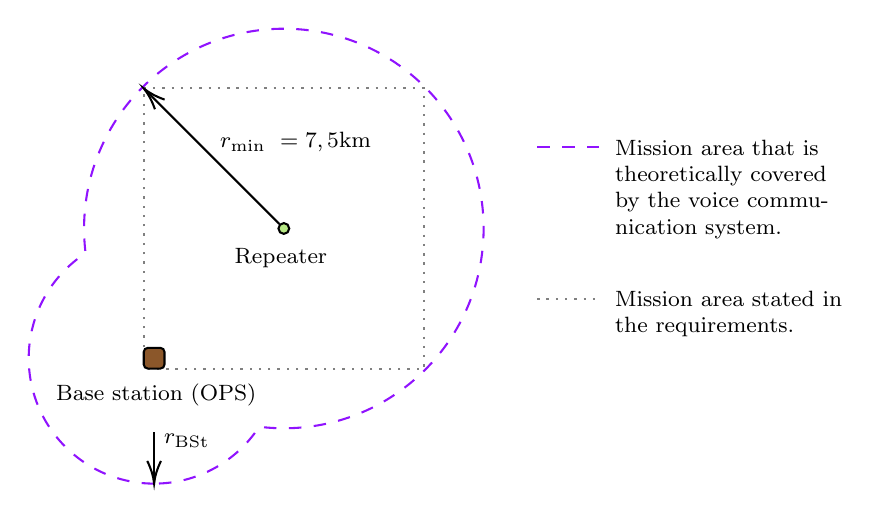
\begin{tikzpicture}[x=0.75pt,y=0.75pt,yscale=-1,xscale=1]
%uncomment if require: \path (0,409); %set diagram left start at 0, and has height of 409

%Shape: Rectangle [id:dp12443341375434458] 
\draw  [color={rgb, 255:red, 128; green, 128; blue, 128 }  ,draw opacity=1 ][dash pattern={on 0.84pt off 2.51pt}] (105.42,168.75) -- (240.42,168.75) -- (240.42,303.75) -- (105.42,303.75) -- cycle ;
%Shape: Path Data [id:dp8368288281183056] 
\draw  [color={rgb, 255:red, 144; green, 19; blue, 254 }  ,draw opacity=1 ][dash pattern={on 4.5pt off 4.5pt}] (110.42,359.17) .. controls (77.05,359.17) and (50,332.12) .. (50,298.75) .. controls (50,277.57) and (60.9,258.93) .. (77.4,248.14) .. controls (76.92,244.24) and (76.67,240.28) .. (76.67,236.25) .. controls (76.67,183.09) and (119.77,140) .. (172.92,140) .. controls (226.08,140) and (269.17,183.09) .. (269.17,236.25) .. controls (269.17,289.41) and (226.08,332.5) .. (172.92,332.5) .. controls (168.9,332.5) and (164.93,332.25) .. (161.04,331.77) .. controls (150.25,348.27) and (131.61,359.17) .. (110.42,359.17) -- cycle ;
%Rounded Rect [id:dp41901798669291956] 
\draw  [fill={rgb, 255:red, 139; green, 87; blue, 42 }  ,fill opacity=1 ] (105.42,295.75) .. controls (105.42,294.65) and (106.32,293.75) .. (107.42,293.75) -- (113.42,293.75) .. controls (114.53,293.75) and (115.42,294.65) .. (115.42,295.75) -- (115.42,301.75) .. controls (115.42,302.85) and (114.53,303.75) .. (113.42,303.75) -- (107.42,303.75) .. controls (106.32,303.75) and (105.42,302.85) .. (105.42,301.75) -- cycle ;
%Straight Lines [id:da8105217749265208] 
\draw    (110.42,357.17) -- (110.42,334.17) ;
\draw [shift={(110.42,359.17)}, rotate = 270] [color={rgb, 255:red, 0; green, 0; blue, 0 }  ][line width=0.75]    (10.93,-3.29) .. controls (6.95,-1.4) and (3.31,-0.3) .. (0,0) .. controls (3.31,0.3) and (6.95,1.4) .. (10.93,3.29)   ;
%Straight Lines [id:da3146532721436186] 
\draw    (106.84,170.16) -- (170.74,234.06) ;
\draw [shift={(105.42,168.75)}, rotate = 45] [color={rgb, 255:red, 0; green, 0; blue, 0 }  ][line width=0.75]    (10.93,-3.29) .. controls (6.95,-1.4) and (3.31,-0.3) .. (0,0) .. controls (3.31,0.3) and (6.95,1.4) .. (10.93,3.29)   ;
%Shape: Circle [id:dp5997567206989125] 
\draw  [fill={rgb, 255:red, 184; green, 233; blue, 134 }  ,fill opacity=1 ] (170.32,236.25) .. controls (170.32,234.81) and (171.49,233.65) .. (172.92,233.65) .. controls (174.36,233.65) and (175.52,234.81) .. (175.52,236.25) .. controls (175.52,237.69) and (174.36,238.85) .. (172.92,238.85) .. controls (171.49,238.85) and (170.32,237.69) .. (170.32,236.25) -- cycle ;
%Straight Lines [id:da1970463822196904] 
\draw [color={rgb, 255:red, 144; green, 19; blue, 254 }  ,draw opacity=1 ] [dash pattern={on 4.5pt off 4.5pt}]  (295,197) -- (325,197) ;

%Straight Lines [id:da2827334971957638] 
\draw [color={rgb, 255:red, 128; green, 128; blue, 128 }  ,draw opacity=1 ] [dash pattern={on 0.84pt off 2.51pt}]  (295,270) -- (325,270) ;


% Text Node
\draw (331,192) node [anchor=north west][inner sep=0.75pt]  [font=\footnotesize] [align=left] {Mission area that is \\theoretically covered\\by the voice commu-\\nication system. };
% Text Node
\draw (61.74,309.44) node [anchor=north west][inner sep=0.75pt]  [font=\footnotesize] [align=left] {Base station (OPS)};
% Text Node
\draw (147.74,244.44) node [anchor=north west][inner sep=0.75pt]  [font=\footnotesize] [align=left] {Repeater};
% Text Node
\draw (113.74,333.84) node [anchor=north west][inner sep=0.75pt]  [font=\footnotesize]  {$r_{\mathrm{BSt}}$};
% Text Node
\draw (140.74,188.46) node [anchor=north west][inner sep=0.75pt]  [font=\footnotesize]  {$r_{\mathrm{min}} \ =7,5\mathrm{km}$};
% Text Node
\draw (331,265) node [anchor=north west][inner sep=0.75pt]  [font=\footnotesize] [align=left] {Mission area stated in\\the requirements.};


\end{tikzpicture}

	\caption{Top view of the mission area covered by the voice communication system.}
	\label{fig:tikz_range}
\end{figure}
Figure \ref{fig:tikz_range} shows the top view of the mission area that is theoretically covered by the voice communication system \cite{Lange:1992}. The border of the mission area covered is illustrated with the dashed purple line. In it, the brown rounded square represents the base station, the green dot represents the repeater and the gray dotted square represents the mission area specified by the system requiremnts. According to these requiremnts the minimum radius is $r_\mathrm{min} = 7,5\mathrm{km}$, as a total mission area of approximately $10\mathrm{km}$ by $10\mathrm{km}$ has to be covered. Furthermore, the system was designed in such a way that the requiremnts are met for the least powerful radio device. 

Since the base station, like the repeater, uses an omnidirectional antenna, the participants of the voice communication system also have reception in an area with a radius $r_\mathrm{BSt}$ in $\left(\mathrm{m}\right)$ around it. By transforming the equation (\ref{eq:plane_earth_approx_db}) and assuming that the fade margin of the least powerful radio device stays the same for the entire coverage area, $r_\mathrm{BSt}$  can be calculated.\footnote{In the equation (\ref{eq:plane_earth_approx_db}), $r_\mathrm{BSt}$ corresponds to the distance $d$.} Although this extends the mission area, it must be taken into account that it may interfere with a neighboring radio system.

In the following subsections each part of the voice communication system will be introduced.

\subsection{Base station radio infrastructure}
The task of the base station crew is to monitor and coordinate both an ongoing mission and the on-site support crew. It is thus the central link of the voice communication system. The base station radio infrastructure is supplied by electrical energy from the local power grid and it consists of a Motorola Mototrbo DM 2600 mobile radio, a Diawa CN-501VN cross needle VSWR \& power meter to monitor the VSWR of the antenna feed line and detect possible errors, a Diamond SP1000 lightning arrester to protect the base station crew, the DM 2600 and the CN-501VN from the consequences of a lightning strike\footnote{It is not recommended to use the voice communication system in situations where lightning strikes may occur.} and a Diamond BC-101 VHF fixed station antenna. Besides that, several adapters and coaxial cables with different lengths $l$ in $\left(\mathrm{m}\right)$ are used to connect these devices and components with each other. 
\begin{figure}[h!]
	\centering
	

\tikzset{every picture/.style={line width=0.75pt}} %set default line width to 0.75pt        

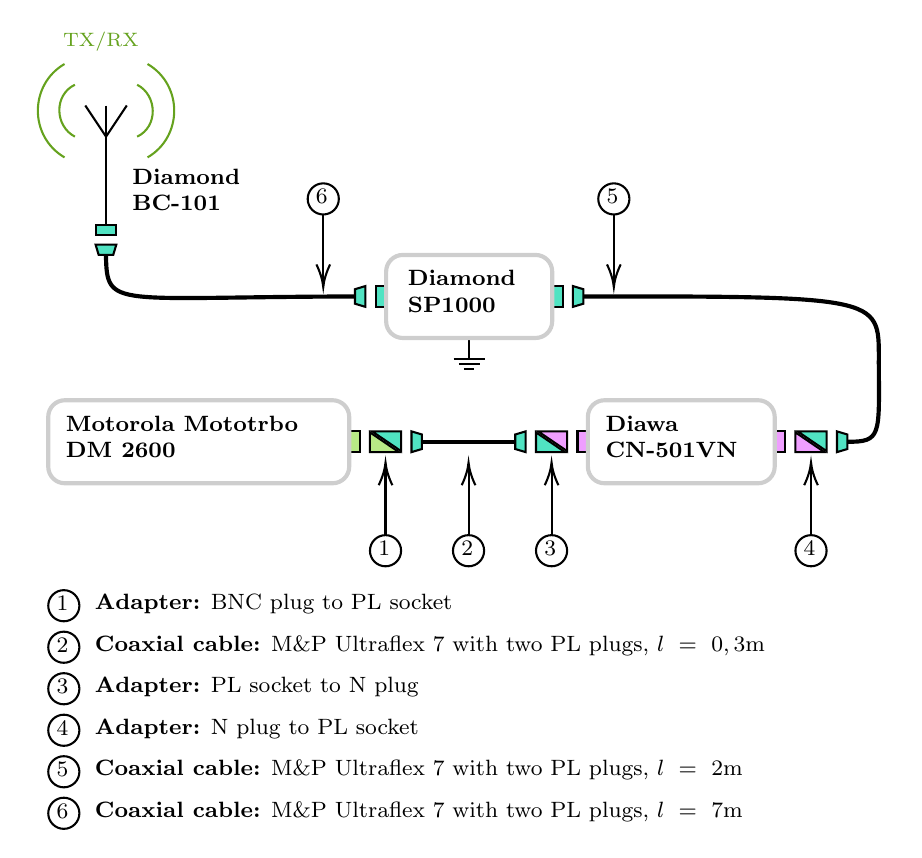
\begin{tikzpicture}[x=0.75pt,y=0.75pt,yscale=-1,xscale=1]
%uncomment if require: \path (0,479); %set diagram left start at 0, and has height of 479

%Straight Lines [id:da5218826641526857] 
\draw    (322.8,185) -- (322.8,195) ;
%Shape: Rectangle [id:dp3707976877259427] 
\draw  [fill={rgb, 255:red, 80; green, 227; blue, 194 }  ,fill opacity=1 ] (362.8,160) -- (367.8,160) -- (367.8,170) -- (362.8,170) -- cycle ;
%Shape: Rectangle [id:dp10664709959227037] 
\draw  [fill={rgb, 255:red, 80; green, 227; blue, 194 }  ,fill opacity=1 ] (277.8,160) -- (282.8,160) -- (282.8,170) -- (277.8,170) -- cycle ;
%Rounded Rect [id:dp527676076956175] 
\draw  [color={rgb, 255:red, 206; green, 206; blue, 206 }  ,draw opacity=1 ][line width=1.5]  (282.8,153) .. controls (282.8,148.58) and (286.38,145) .. (290.8,145) -- (354.8,145) .. controls (359.22,145) and (362.8,148.58) .. (362.8,153) -- (362.8,177) .. controls (362.8,181.42) and (359.22,185) .. (354.8,185) -- (290.8,185) .. controls (286.38,185) and (282.8,181.42) .. (282.8,177) -- cycle ;

%Straight Lines [id:da6289021026698145] 
\draw    (147.84,73) -- (147.84,133) ;
%Straight Lines [id:da47703805930667476] 
\draw    (137.84,73) -- (147.84,88) ;
%Straight Lines [id:da4218266835017126] 
\draw    (147.84,88) -- (157.84,73) ;
%Curve Lines [id:da5241031222048758] 
\draw [color={rgb, 255:red, 101; green, 162; blue, 30 }  ,draw opacity=1 ]   (162.84,63) .. controls (172.56,68) and (173.13,83.14) .. (162.84,88) ;
%Curve Lines [id:da3821737885384662] 
\draw [color={rgb, 255:red, 101; green, 162; blue, 30 }  ,draw opacity=1 ]   (167.84,53) .. controls (185.09,63.13) and (184.84,88.13) .. (167.84,98) ;

%Curve Lines [id:da3538255270661379] 
\draw [color={rgb, 255:red, 101; green, 162; blue, 30 }  ,draw opacity=1 ]   (132.84,88) .. controls (123.13,83) and (122.56,67.86) .. (132.84,63) ;
%Curve Lines [id:da889352578619292] 
\draw [color={rgb, 255:red, 101; green, 162; blue, 30 }  ,draw opacity=1 ]   (127.84,98) .. controls (110.59,87.88) and (110.84,62.87) .. (127.84,53) ;

%Shape: Rectangle [id:dp9150249297100126] 
\draw  [fill={rgb, 255:red, 80; green, 227; blue, 194 }  ,fill opacity=1 ] (142.84,130.5) -- (152.84,130.5) -- (152.84,135.5) -- (142.84,135.5) -- cycle ;
%Shape: Trapezoid [id:dp6261372647556653] 
\draw  [fill={rgb, 255:red, 80; green, 227; blue, 194 }  ,fill opacity=1 ][line width=0.75]  (152.8,140) -- (151.3,145) -- (144.3,145) -- (142.8,140) -- cycle ;
%Shape: Trapezoid [id:dp4286379946581531] 
\draw  [fill={rgb, 255:red, 80; green, 227; blue, 194 }  ,fill opacity=1 ][line width=0.75]  (272.8,170) -- (267.8,168.5) -- (267.8,161.5) -- (272.8,160) -- cycle ;
%Curve Lines [id:da8045163154695201] 
\draw [line width=1.5]    (147.8,145) .. controls (148.3,171.25) and (150.3,165.25) .. (267.8,165) ;
%Straight Lines [id:da19181563997268603] 
\draw    (315.3,195) -- (330.3,195) ;
%Straight Lines [id:da020619477423114985] 
\draw    (317.8,197.5) -- (327.8,197.5) ;
%Straight Lines [id:da9009961872255909] 
\draw    (320.3,200) -- (325.3,200) ;
%Shape: Rectangle [id:dp35598711466417887] 
\draw  [fill={rgb, 255:red, 239; green, 158; blue, 255 }  ,fill opacity=1 ] (470,230) -- (475,230) -- (475,240) -- (470,240) -- cycle ;
%Shape: Rectangle [id:dp4791882432942969] 
\draw  [fill={rgb, 255:red, 239; green, 158; blue, 255 }  ,fill opacity=1 ] (375,230) -- (380,230) -- (380,240) -- (375,240) -- cycle ;
%Shape: Rectangle [id:dp2776872187237942] 
\draw  [fill={rgb, 255:red, 184; green, 233; blue, 134 }  ,fill opacity=1 ] (265,230) -- (270,230) -- (270,240) -- (265,240) -- cycle ;
%Rounded Rect [id:dp5113702121898573] 
\draw  [color={rgb, 255:red, 206; green, 206; blue, 206 }  ,draw opacity=1 ][line width=1.5]  (120,223) .. controls (120,218.58) and (123.58,215) .. (128,215) -- (257,215) .. controls (261.42,215) and (265,218.58) .. (265,223) -- (265,247) .. controls (265,251.42) and (261.42,255) .. (257,255) -- (128,255) .. controls (123.58,255) and (120,251.42) .. (120,247) -- cycle ;

%Straight Lines [id:da5653713287945248] 
\draw [line width=1.5]    (300,235) -- (345,235) ;
%Shape: Trapezoid [id:dp6827000741886373] 
\draw  [fill={rgb, 255:red, 80; green, 227; blue, 194 }  ,fill opacity=1 ][line width=0.75]  (295,230) -- (300,231.5) -- (300,238.5) -- (295,240) -- cycle ;
%Shape: Trapezoid [id:dp5551727639514186] 
\draw  [fill={rgb, 255:red, 80; green, 227; blue, 194 }  ,fill opacity=1 ][line width=0.75]  (350,240) -- (345,238.5) -- (345,231.5) -- (350,230) -- cycle ;

%Shape: Right Triangle [id:dp6567087371846239] 
\draw  [fill={rgb, 255:red, 184; green, 233; blue, 134 }  ,fill opacity=1 ] (275,230.48) -- (288.98,240) -- (275,240) -- cycle ;
%Shape: Right Triangle [id:dp6439631638146213] 
\draw  [fill={rgb, 255:red, 80; green, 227; blue, 194 }  ,fill opacity=1 ] (290,239.52) -- (276.02,230) -- (290,230) -- cycle ;

%Shape: Right Triangle [id:dp7065836348516847] 
\draw  [fill={rgb, 255:red, 80; green, 227; blue, 194 }  ,fill opacity=1 ] (355,230.48) -- (368.98,240) -- (355,240) -- cycle ;
%Shape: Right Triangle [id:dp6791715198368578] 
\draw  [fill={rgb, 255:red, 239; green, 158; blue, 255 }  ,fill opacity=1 ] (370,239.52) -- (356.02,230) -- (370,230) -- cycle ;

%Rounded Rect [id:dp5242124209678602] 
\draw  [color={rgb, 255:red, 206; green, 206; blue, 206 }  ,draw opacity=1 ][line width=1.5]  (380,223) .. controls (380,218.58) and (383.58,215) .. (388,215) -- (462,215) .. controls (466.42,215) and (470,218.58) .. (470,223) -- (470,247) .. controls (470,251.42) and (466.42,255) .. (462,255) -- (388,255) .. controls (383.58,255) and (380,251.42) .. (380,247) -- cycle ;
%Shape: Right Triangle [id:dp9024696438630258] 
\draw  [fill={rgb, 255:red, 80; green, 227; blue, 194 }  ,fill opacity=1 ] (495,239.52) -- (481.02,230) -- (495,230) -- cycle ;
%Shape: Right Triangle [id:dp3027647623967811] 
\draw  [fill={rgb, 255:red, 239; green, 158; blue, 255 }  ,fill opacity=1 ] (480,230.48) -- (493.98,240) -- (480,240) -- cycle ;

%Curve Lines [id:da5556976336058517] 
\draw [line width=1.5]    (375.3,165) .. controls (526.33,164.83) and (520,165.25) .. (520.17,198.54) .. controls (520.34,231.82) and (521.33,235.17) .. (505,235) ;
%Shape: Trapezoid [id:dp7689909076073862] 
\draw  [fill={rgb, 255:red, 80; green, 227; blue, 194 }  ,fill opacity=1 ][line width=0.75]  (372.8,160) -- (377.8,161.5) -- (377.8,168.5) -- (372.8,170) -- cycle ;
%Shape: Trapezoid [id:dp5759023250736097] 
\draw  [fill={rgb, 255:red, 80; green, 227; blue, 194 }  ,fill opacity=1 ][line width=0.75]  (500,230) -- (505,231.5) -- (505,238.5) -- (500,240) -- cycle ;
%Straight Lines [id:da0668317935629783] 
\draw    (282.5,280) -- (282.5,247) ;
\draw [shift={(282.5,245)}, rotate = 450] [color={rgb, 255:red, 0; green, 0; blue, 0 }  ][line width=0.75]    (10.93,-3.29) .. controls (6.95,-1.4) and (3.31,-0.3) .. (0,0) .. controls (3.31,0.3) and (6.95,1.4) .. (10.93,3.29)   ;
%Shape: Circle [id:dp8618966688089644] 
\draw   (275,287.5) .. controls (275,283.36) and (278.36,280) .. (282.5,280) .. controls (286.64,280) and (290,283.36) .. (290,287.5) .. controls (290,291.64) and (286.64,295) .. (282.5,295) .. controls (278.36,295) and (275,291.64) .. (275,287.5) -- cycle ;


%Shape: Circle [id:dp06491171475414959] 
\draw   (315,287.5) .. controls (315,283.36) and (318.36,280) .. (322.5,280) .. controls (326.64,280) and (330,283.36) .. (330,287.5) .. controls (330,291.64) and (326.64,295) .. (322.5,295) .. controls (318.36,295) and (315,291.64) .. (315,287.5) -- cycle ;

%Straight Lines [id:da006440625484793738] 
\draw    (322.5,280) -- (322.5,247) ;
\draw [shift={(322.5,245)}, rotate = 450] [color={rgb, 255:red, 0; green, 0; blue, 0 }  ][line width=0.75]    (10.93,-3.29) .. controls (6.95,-1.4) and (3.31,-0.3) .. (0,0) .. controls (3.31,0.3) and (6.95,1.4) .. (10.93,3.29)   ;

%Shape: Circle [id:dp9167743181241499] 
\draw   (355,287.5) .. controls (355,283.36) and (358.36,280) .. (362.5,280) .. controls (366.64,280) and (370,283.36) .. (370,287.5) .. controls (370,291.64) and (366.64,295) .. (362.5,295) .. controls (358.36,295) and (355,291.64) .. (355,287.5) -- cycle ;

%Straight Lines [id:da48094261953448303] 
\draw    (362.5,280) -- (362.5,247) ;
\draw [shift={(362.5,245)}, rotate = 450] [color={rgb, 255:red, 0; green, 0; blue, 0 }  ][line width=0.75]    (10.93,-3.29) .. controls (6.95,-1.4) and (3.31,-0.3) .. (0,0) .. controls (3.31,0.3) and (6.95,1.4) .. (10.93,3.29)   ;

%Shape: Circle [id:dp1939511278206627] 
\draw   (480,287.5) .. controls (480,283.36) and (483.36,280) .. (487.5,280) .. controls (491.64,280) and (495,283.36) .. (495,287.5) .. controls (495,291.64) and (491.64,295) .. (487.5,295) .. controls (483.36,295) and (480,291.64) .. (480,287.5) -- cycle ;

%Straight Lines [id:da3351576985038338] 
\draw    (487.5,280) -- (487.5,247) ;
\draw [shift={(487.5,245)}, rotate = 450] [color={rgb, 255:red, 0; green, 0; blue, 0 }  ][line width=0.75]    (10.93,-3.29) .. controls (6.95,-1.4) and (3.31,-0.3) .. (0,0) .. controls (3.31,0.3) and (6.95,1.4) .. (10.93,3.29)   ;

%Shape: Circle [id:dp5129779571773962] 
\draw   (385,118) .. controls (385,113.86) and (388.36,110.5) .. (392.5,110.5) .. controls (396.64,110.5) and (400,113.86) .. (400,118) .. controls (400,122.14) and (396.64,125.5) .. (392.5,125.5) .. controls (388.36,125.5) and (385,122.14) .. (385,118) -- cycle ;

%Straight Lines [id:da6621400269321598] 
\draw    (392.5,158.5) -- (392.5,125.5) ;
\draw [shift={(392.5,160.5)}, rotate = 270] [color={rgb, 255:red, 0; green, 0; blue, 0 }  ][line width=0.75]    (10.93,-3.29) .. controls (6.95,-1.4) and (3.31,-0.3) .. (0,0) .. controls (3.31,0.3) and (6.95,1.4) .. (10.93,3.29)   ;

%Shape: Circle [id:dp7977203271441822] 
\draw   (245,118) .. controls (245,113.86) and (248.36,110.5) .. (252.5,110.5) .. controls (256.64,110.5) and (260,113.86) .. (260,118) .. controls (260,122.14) and (256.64,125.5) .. (252.5,125.5) .. controls (248.36,125.5) and (245,122.14) .. (245,118) -- cycle ;

%Straight Lines [id:da2162256591147207] 
\draw    (252.5,158.5) -- (252.5,125.5) ;
\draw [shift={(252.5,160.5)}, rotate = 270] [color={rgb, 255:red, 0; green, 0; blue, 0 }  ][line width=0.75]    (10.93,-3.29) .. controls (6.95,-1.4) and (3.31,-0.3) .. (0,0) .. controls (3.31,0.3) and (6.95,1.4) .. (10.93,3.29)   ;

%Shape: Circle [id:dp24834021243597504] 
\draw   (120,314) .. controls (120,309.86) and (123.36,306.5) .. (127.5,306.5) .. controls (131.64,306.5) and (135,309.86) .. (135,314) .. controls (135,318.14) and (131.64,321.5) .. (127.5,321.5) .. controls (123.36,321.5) and (120,318.14) .. (120,314) -- cycle ;

%Shape: Circle [id:dp7233992369838149] 
\draw   (120,334) .. controls (120,329.86) and (123.36,326.5) .. (127.5,326.5) .. controls (131.64,326.5) and (135,329.86) .. (135,334) .. controls (135,338.14) and (131.64,341.5) .. (127.5,341.5) .. controls (123.36,341.5) and (120,338.14) .. (120,334) -- cycle ;

%Shape: Circle [id:dp6313697664795326] 
\draw   (120,354) .. controls (120,349.86) and (123.36,346.5) .. (127.5,346.5) .. controls (131.64,346.5) and (135,349.86) .. (135,354) .. controls (135,358.14) and (131.64,361.5) .. (127.5,361.5) .. controls (123.36,361.5) and (120,358.14) .. (120,354) -- cycle ;

%Shape: Circle [id:dp03435814103609336] 
\draw   (120,374) .. controls (120,369.86) and (123.36,366.5) .. (127.5,366.5) .. controls (131.64,366.5) and (135,369.86) .. (135,374) .. controls (135,378.14) and (131.64,381.5) .. (127.5,381.5) .. controls (123.36,381.5) and (120,378.14) .. (120,374) -- cycle ;

%Shape: Circle [id:dp003390866078124999] 
\draw   (120,394) .. controls (120,389.86) and (123.36,386.5) .. (127.5,386.5) .. controls (131.64,386.5) and (135,389.86) .. (135,394) .. controls (135,398.14) and (131.64,401.5) .. (127.5,401.5) .. controls (123.36,401.5) and (120,398.14) .. (120,394) -- cycle ;

%Shape: Circle [id:dp7433181145978278] 
\draw   (120,414) .. controls (120,409.86) and (123.36,406.5) .. (127.5,406.5) .. controls (131.64,406.5) and (135,409.86) .. (135,414) .. controls (135,418.14) and (131.64,421.5) .. (127.5,421.5) .. controls (123.36,421.5) and (120,418.14) .. (120,414) -- cycle ;



% Text Node
\draw (159,102) node [anchor=north west][inner sep=0.75pt]  [font=\footnotesize] [align=left] {\textbf{Diamond }\\\textbf{BC-101}};
% Text Node
\draw (127,221) node [anchor=north west][inner sep=0.75pt]  [font=\footnotesize] [align=left] {\textbf{Motorola Mototrbo}\\\textbf{DM 2600}};
% Text Node
\draw (387,221) node [anchor=north west][inner sep=0.75pt]  [font=\footnotesize] [align=left] {\textbf{Diawa}\\\textbf{CN-501VN}};
% Text Node
\draw (291.8,151) node [anchor=north west][inner sep=0.75pt]  [font=\footnotesize] [align=left] {\textbf{Diamond}\\\textbf{SP1000}};
% Text Node
\draw (125.69,36) node [anchor=north west][inner sep=0.75pt]  [font=\scriptsize,color={rgb, 255:red, 101; green, 162; blue, 30 }  ,opacity=1 ] [align=left] {TX/RX};
% Text Node
\draw (277.5,281.5) node [anchor=north west][inner sep=0.75pt]  [font=\footnotesize] [align=left] {1};
% Text Node
\draw (317.5,281.5) node [anchor=north west][inner sep=0.75pt]  [font=\footnotesize] [align=left] {2};
% Text Node
\draw (357.5,281.5) node [anchor=north west][inner sep=0.75pt]  [font=\footnotesize] [align=left] {3};
% Text Node
\draw (482.5,281.5) node [anchor=north west][inner sep=0.75pt]  [font=\footnotesize] [align=left] {4};
% Text Node
\draw (387.5,112) node [anchor=north west][inner sep=0.75pt]  [font=\footnotesize] [align=left] {5};
% Text Node
\draw (247.5,112) node [anchor=north west][inner sep=0.75pt]  [font=\footnotesize] [align=left] {6};
% Text Node
\draw (122.5,308) node [anchor=north west][inner sep=0.75pt]  [font=\footnotesize] [align=left] {1};
% Text Node
\draw (122.5,328) node [anchor=north west][inner sep=0.75pt]  [font=\footnotesize] [align=left] {2};
% Text Node
\draw (122.5,348) node [anchor=north west][inner sep=0.75pt]  [font=\footnotesize] [align=left] {3};
% Text Node
\draw (122.5,368) node [anchor=north west][inner sep=0.75pt]  [font=\footnotesize] [align=left] {4};
% Text Node
\draw (122.5,388) node [anchor=north west][inner sep=0.75pt]  [font=\footnotesize] [align=left] {5};
% Text Node
\draw (122.5,408) node [anchor=north west][inner sep=0.75pt]  [font=\footnotesize] [align=left] {6};
% Text Node
\draw (141,307) node [anchor=north west][inner sep=0.75pt]  [font=\footnotesize] [align=left] {\textbf{Adapter:} BNC plug to PL socket};
% Text Node
\draw (141,327) node [anchor=north west][inner sep=0.75pt]  [font=\footnotesize] [align=left] {\textbf{Coaxial cable:} M\&P Ultraflex 7 with two PL plugs, $\displaystyle l\ =\ 0,3\mathrm{m}$};
% Text Node
\draw (141,347) node [anchor=north west][inner sep=0.75pt]  [font=\footnotesize] [align=left] {\textbf{Adapter:} PL socket to N plug};
% Text Node
\draw (141,367) node [anchor=north west][inner sep=0.75pt]  [font=\footnotesize] [align=left] {\textbf{Adapter:} N plug to PL socket};
% Text Node
\draw (141,387) node [anchor=north west][inner sep=0.75pt]  [font=\footnotesize] [align=left] {\textbf{Coaxial cable:} M\&P Ultraflex 7 with two PL plugs, $\displaystyle l\ =\ 2\mathrm{m}$};
% Text Node
\draw (141,407) node [anchor=north west][inner sep=0.75pt]  [font=\footnotesize] [align=left] {\textbf{Coaxial cable:} M\&P Ultraflex 7 with two PL plugs, $\displaystyle l\ =\ 7\mathrm{m}$};


\end{tikzpicture}

	\caption{Schematic structure of the base station radio infrastructure.}
	\label{fig:tikz_base_camp_radio}
\end{figure}
Figure \ref{fig:tikz_base_camp_radio} provides an illustration. There are gaps between the devices and components to make the schematic structure easier to read.\footnote{In practice these are connected.} Green connectors represent a BNC plug or socket, turquoise connectors represent a PL plug or socket and pink connectors represent a N plug or socket. For more information on whether it is a socket or a plug, see figure \ref{fig:tikz_base_camp_radio} and tables \ref{tab:table_dm2600_specs} through \ref{tab:table_ultraflex_7_specs}. Adapters -- such as \circled{\footnotesize{1}} and \circled{\footnotesize{3}} -- are characterized by a rectangle with a diagonal drawn in. The colors in the resulting right-angled triangles indicate which connectors an adapter has. Coaxial cables are drawn with a thicker line and trapezoids as connectors -- for example \circled{\footnotesize{2}}, \circled{\footnotesize{5}} and \circled{\footnotesize{6}}. Because the coaxial cables were delivered without connectors, they were installed afterwards. The connectors of the DM 2600, Diawa CN-501VN, Diamond SP1000 and Diamond BC-101 are marked by a small rectangle which is in direct contact with the associated device or component. These have factory-installed connectors which their data sheets already take into account.

From the data sheet of the DM 2600, from which an excerpt is provided in table \ref{tab:table_dm2600_specs}, it can be seen that its maximum transmission power is $25\mathrm{W}$ and its sensitivity -- in the worst case -- is $0,25\mathrm{\mu V}$.
\begin{table}[h!]
	\centering
	\footnotesize
\begin{tabular}{|l|c|}
	\hline
	\multicolumn{2}{|c|}{\textbf{Motorola Mototrbo DM 2600 (VHF digital) specifications}} \\
	\hline
 	Frequency & $136\mathrm{MHz}$ to $174\mathrm{MHz}$ \\
	System impedance & $50\Omega$\\
 	Dimensions $\mathrm{(H \times W \times D)}$ & $44 \times 169 \times 134 \mathrm{mm}$ \\%
 	Mass & $1,3\mathrm{kg}$ \\%
	Power supply & $13,2\mathrm{VDC}$ (nominal) ($10,8$ to $15,6\mathrm{VDC}$) \\
	Current standby & $0,81\mathrm{A}$ (max.) \\
	Current RX & $2\mathrm{A}$ (max.) \\
	Current TX & $11\mathrm{A}$ (max.) \\
	Operating temperature & $-30^\circ \mathrm{C}$ to $60^\circ \mathrm{C}$ \\
	Storage temperature & $-40^\circ \mathrm{C}$ to $85^\circ \mathrm{C}$ \\
	RX sensitivity 5\% BER: & $0,25\mathrm{\mu V}$ ($0,19\mathrm{\mu V}$ typical) \\
	TX power output & $1\mathrm{W}$ to $25\mathrm{W}$ \\
	Connector & BNC socket\\
	\hline
\end{tabular}
	\caption{Excerpt from the data sheet of the Motorola Mototrbo DM 2600 mobile radio. \cite{DM2600:2013}}
	\label{tab:table_dm2600_specs}
\end{table}
Its maximum transmission and minimum required reception power therefore follow to:
\begin{equation} \label{eq:power_BSt_tx}
	\centering
	P_\mathrm{T,dBW} =  10\mathrm{dBW} \cdot \log_{10} \left( \dfrac{25\mathrm{W}}{1\mathrm{W}} \right) = 13,979\mathrm{dBW}\text{,}
\end{equation}
\begin{equation} \label{eq:power_BSt_min}
	\centering
	P_\mathrm{min,dBW} = 10\mathrm{dBW} \cdot \log_{10} \left( \dfrac{\left(0,25\cdot10^{-6}\mathrm{V}\right)^2}{50\Omega} \right) = -149,031\mathrm{dBW}\text{.}
\end{equation}

It is assumed that the CN-501VN will not cause any loss or gain in the antenna feed line as its data sheet does not contain any specifications on this matter. An excerpt of said data sheet can be seen in the table \ref{tab:table_daiwa_cn_501}.
\begin{table}[h!]
	\centering
	\footnotesize
\begin{tabular}{|l|c|}
	\hline
	\multicolumn{2}{|c|}{\textbf{Daiwa CN-501VN specifications}} \\
	\hline
 	Frequency & $140\mathrm{MHz}$ to $525\mathrm{MHz}$ \\
	Input/Output impedance & $50\Omega$\\
	Dimensions $\mathrm{(H \times W \times D)}$ & $80 \times 155 \times 100 \mathrm{mm}$ \\%
 	Weight& $0,67\mathrm{kg}$ \\%
	Power range & $20\mathrm{W}/200\mathrm{W}$ (forward) \\
	Power rating & $200\mathrm{W}$ ($140\mathrm{MHz}$ to $525\mathrm{MHz}$) \\
	Tolerance & $\pm10\%$ at full scale \\
	VSWR measurement range & $1$ to $\infty$\\
	VSWR detection sensitivity & $200\mathrm{W}$ (min.)\\
	Connector & $2 \times \text{N socket}$ \\
	\hline
\end{tabular}
	\caption{Excerpt from the data sheet of the Daiwa CN-501VN cross needle VSWR \& power meter.\cite{Daiwa-industry-co.:2016}}
	\label{tab:table_daiwa_cn_501}
\end{table}

The SP1000 has an insertion loss of less than $0,2\mathrm{dB}$ and a VSWR of less than $1,2$ as shown in the table \ref{tab:table_lightning_arrestor_specs}.
\begin{table}[h!]
	\centering
	\footnotesize
\begin{tabular}{|l|c|}
	\hline
	\multicolumn{2}{|c|}{\textbf{Diamond SP1000 specification}} \\
	\hline
 	Frequency range & \numrange{0}{1000}$\mathrm{MHz}$ \\ % DC -> 0Hz 
 	Impedance & $50\Omega$ \\
 	VSWR & $< 1,2$ \\
	Insertion loss & $< 0,2\mathrm{dB}$ \\
 	Max. power rating & $400\mathrm{W}$ \\
	Impulse wave discharge voltage & $1000\mathrm{V}$ \\
	Impulse wave discharge current & $6000\mathrm{A}$ \\
	Impulse wave retention voltage & $350\mathrm{VDC} \pm 20\%$ \\
	Insulating resistance ($100\mathrm{VDC}$) & $> 10000\mathrm{M}\Omega$ \\
	Connector & $2 \times \text{PL socket}$ \\
	\hline
\end{tabular}
	\caption{Excerpt from the data sheet of the Diamond SP1000 lightning arrester. \cite{SP1000:2020}}
	\label{tab:table_lightning_arrestor_specs}
\end{table}
If now the worst case is assumed -- which means that the insertion loss is exactly $0,2\mathrm{dB}$ and the VSWR is exactly $1,2$ -- then the total loss caused by this component is the sum of the insertion and the mismatch loss:
\begin{equation} \label{eq:losses_BSt_arr}
	\centering
	L_\mathrm{arr,dB} = 0,2\mathrm{dB} - 10\mathrm{dB} \cdot \log_{10} \left(1 - \left(\dfrac{1,2 - 1}{1,2 + 1}\right)^2\right) = 0,236\mathrm{dB}\text{.}
\end{equation}

As can be seen in the table \ref{tab:table_bc101_specs}, the BC-101 has a gain of $G_\mathrm{ant,dBi} = 3,5\mathrm{dBi}$ and a VSWR of less than $1,5$.
\begin{table}[h!]
	\centering
	\footnotesize
\begin{tabular}{|l|c|}
	\hline
	\multicolumn{2}{|c|}{\textbf{Diamond BC-101 specifications}} \\
	\hline
 	Type & 5/8 wave ground plane \\
 	Frequency & $144\mathrm{MHz}$ to $174\mathrm{MHz}$ \\
	Impedance & $50\Omega$\\
	Gain & $3,5\mathrm{dBi}$\\
 	Power rating & $200\mathrm{W}$ (max.) \\
 	VSWR & $< 1,5$ \\
	Weight & $0,86\mathrm{kg}$ \\
	Connector & PL plug \\
	\hline
\end{tabular}
	\caption{Excerpt from the data sheet of the Diamond BC-101 VHF fixed station antenna.\cite{antenna:2020}}
	\label{tab:table_bc101_specs}
\end{table}
With $\mathrm{VSWR} = 1,5$, the mismatch loss in the worst case can be calculated as shown in the equation (\ref{eq:losses_BSt_ant}).
\begin{equation} \label{eq:losses_BSt_ant}
	\centering
	L_\mathrm{ant,dB} = - 10\mathrm{dB} \cdot \log_{10} \left(1 - \left(\dfrac{1,5 - 1}{1,5 + 1}\right)^2\right) = 0,177\mathrm{dB}
\end{equation}
Regarding this antenna, it should also be mentioned that a mast will be made available at the mission site. Therefore, the height of the mast can vary from mission to mission. An antenna, which is set up on a $1\mathrm{m}$ high tripod on a freight container in accordance with ISO 668, has approximately a height of $h _\mathrm{BSt} = 3,6\mathrm{m}$ above the ground. This height is used for the link budget estimation. 

All coaxial cables used for the voice communication system are Messi \& Paoloni Ultraflex 7 coaxial cables. An excerpt of the data sheet of this coaxial cable can be found in the table \ref{tab:table_ultraflex_7_specs} and the attenuation as a function of the frequency -- interpolated with a \MATLAB program -- according to its data sheet, in the figure \ref{fig:image_attenuation_UF7}. 
\begin{table}[h!]
	\centering
	\footnotesize
\begin{tabular}{|l|c|}
	\hline
	\multicolumn{2}{|c|}{\textbf{Messi \& Paoloni Ultraflex 7 specifications}} \\
	\hline
 	Frequency & $1,8\mathrm{MHz}$ to $8000\mathrm{MHz}$ \\
	Impedance & $50\pm3\Omega$ (at $200\mathrm{MHz}$)\\
	Operating temperature & $-40^\circ \mathrm{C}$ to $60^\circ \mathrm{C}$ \\
	Inner conductor resistance & $7,3\Omega\mathrm{km}^{-1}$ \\
	Outer conductor resistance & $9,8\Omega\mathrm{km}^{-1}$ \\
	Capacitance & $75\pm3\mathrm{pFm}^{-1}$ \\
	Power rating & $8000\mathrm{W}$ (peak) \\
	Net. weight & $6,9\mathrm{kg}/100\mathrm{m}$ \\
	Connector & none \\
	\hline
\end{tabular}
	\caption{Excerpt from the data sheet of the Messi \& Poloni Ultraflex 7 coaxial cable. \cite{Paoloni:2021}}
	\label{tab:table_ultraflex_7_specs}
\end{table}
\begin{figure}[h!]
	\centering
  	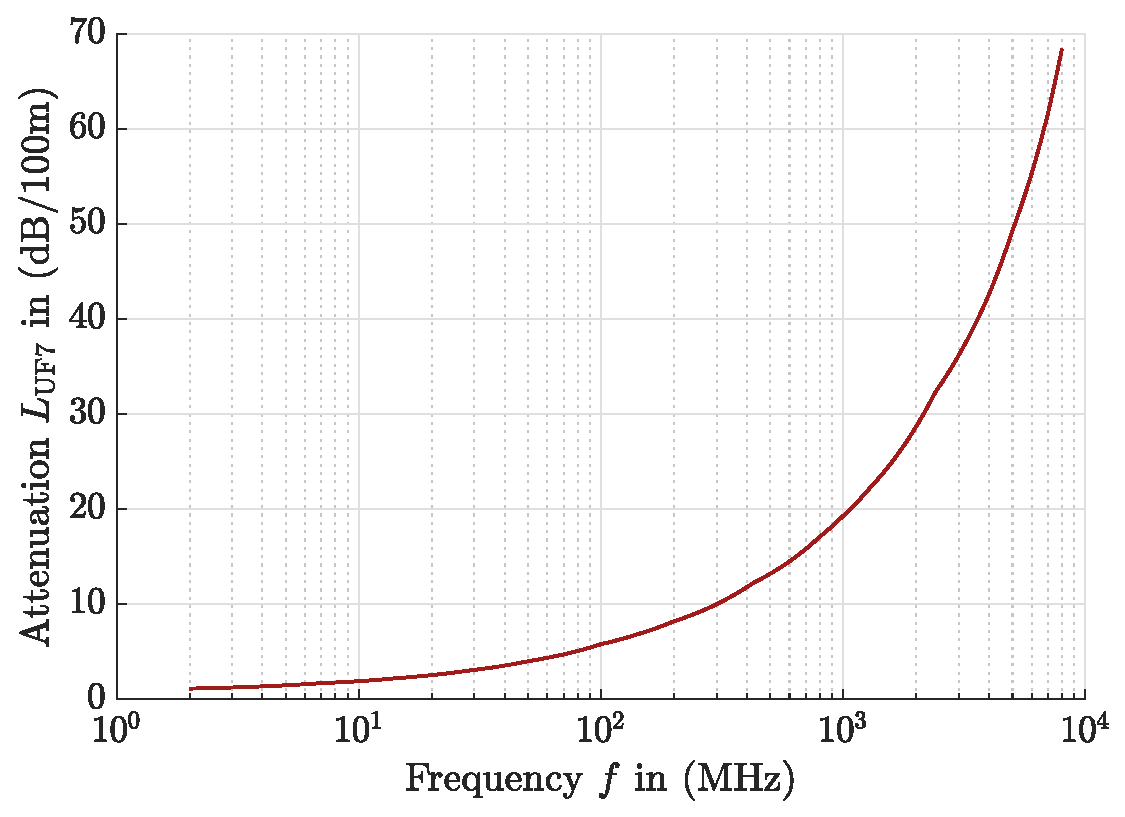
\includegraphics[width = 0.67\textwidth]{image_attenuation_UF7.eps}
  	\caption{Attenuation of the Messi \& Paoloni Ultraflex 7 coaxial cable for $20^\circ \mathrm{C}$. For the frequency $f_\sim = 158,950\mathrm{MHz}$, the attenuation is around $7,2471\mathrm{dB/100m}$. (Recreated from: \cite{Paoloni:2021})}
	\label{fig:image_attenuation_UF7}
\end{figure}
Based on this, an attenuation of $7,2471\mathrm{dB/100m}$ was determined for the frequency $f_\sim = 158,950\mathrm{MHz}$. The cable lengths of the individual coaxial cables in the systems can be taken from the figure \ref{fig:tikz_base_camp_radio}. This results in an insertion loss -- without connectors -- of:
\begin{equation} \label{eq:losses_BSt_coax}
	\centering
	L_\mathrm{coax,dB} = \dfrac{7,2471 \cdot 9,3}{100}\mathrm{dB} = 0,674\mathrm{dB}\text{.}
\end{equation}
It is noted, that $L_\mathrm{coax,dB}$ increases as the cable length increases. It can become significantly greater if the antenna is mounted at a location further away from the base station. 

Regarding the attenuation of the numbered adapters and connectors, which also includes the connectors of the coaxial cables in the figure \ref{fig:tikz_base_camp_radio}, it is assumed that each of these has an attenuation of $0,1 \mathrm{dB}$ \cite{LinkMargin:2016}. With $N_\mathrm{I} = 9$, the total insertion loss caused by the connectors and adapters follows to:
\begin{equation} \label{eq:losses_BSt_conn}
	\centering
	L_\mathrm{conn/adapt,dB} = 0,9\mathrm{dB}\text{.}
\end{equation}
An assumption was made because no data sheets for the adapters and connectors were found. 

From the above, the total loss of the antenna feed line now results in:
\begin{equation} \label{eq:losses_BSt}
	\centering
	L_\mathrm{BSt,dB} = L_\mathrm{arr,dB} + L_\mathrm{ant,dB} + L_\mathrm{coax,dB} + L_\mathrm{conn/adapt,dB} = 1,987\mathrm{dB}\text{.}
\end{equation}








%\textcolor{rgb, 255:red, 80; green, 227; blue, 194 }{turquoise} 




\subsection{Repeater radio infrastructure}
The main task of the repeater is to receive weak signals and to re-transmit them with increased transmission power. Its radio infrastructure is supplied by electrical energy from the self-sufficient energy distribution system, for which the schematic structure is shown in the figure \ref{fig:tikz_rep_energy}. As it can be seen, an AE Solar AE195SMM6-36 PV generator with pre-mounted cables \circled{\footnotesize{A}}, a Victron BlueSolar MPPT 75/10 SCC and an Offgridtec Smart-Pro $12,8\mathrm{V}$ $50\mathrm{Ah}$ $\mathrm{LiFePO}_4$ battery are used. In addition, the cables \circled{\footnotesize{B}} and \circled{\footnotesize{C}}, which are designed for harsh environments, are used to connect these devices.
\begin{figure}[h!]
	\centering
	

\tikzset{every picture/.style={line width=0.75pt}} %set default line width to 0.75pt        

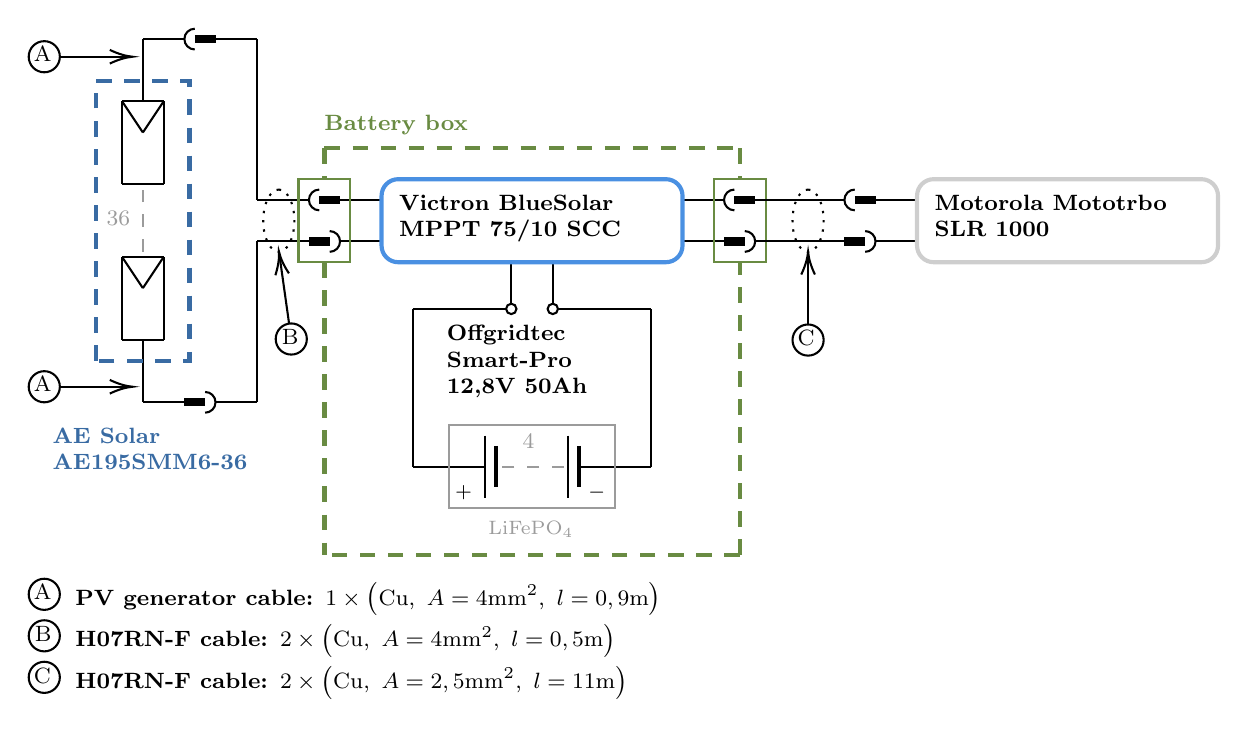
\begin{tikzpicture}[x=0.75pt,y=0.75pt,yscale=-1,xscale=1]
%uncomment if require: \path (0,440); %set diagram left start at 0, and has height of 440

%Straight Lines [id:da11510906097283446] 
\draw    (137,125) -- (162,125) ;
%Straight Lines [id:da5492120144829185] 
\draw    (137,145) -- (162,145) ;
%Straight Lines [id:da5723707691800957] 
\draw    (362,145) -- (342,145) ;
%Straight Lines [id:da24173928983034854] 
\draw    (362,125) -- (342,125) ;
%Straight Lines [id:da7288463432166432] 
\draw [line width=3]    (367,125) -- (377,125) ;
%Shape: Arc [id:dp807105785534799] 
\draw  [draw opacity=0] (367,120) .. controls (367,120) and (367,120) .. (367,120) .. controls (364.24,120) and (362,122.24) .. (362,125) .. controls (362,127.76) and (364.24,130) .. (367,130) -- (367,125) -- cycle ; \draw   (367,120) .. controls (367,120) and (367,120) .. (367,120) .. controls (364.24,120) and (362,122.24) .. (362,125) .. controls (362,127.76) and (364.24,130) .. (367,130) ;

%Straight Lines [id:da8769078095389509] 
\draw [line width=3]    (372,145) -- (362,145) ;
%Shape: Arc [id:dp8109222486657941] 
\draw  [draw opacity=0] (372,150) .. controls (372,150) and (372,150) .. (372,150) .. controls (374.76,150) and (377,147.76) .. (377,145) .. controls (377,142.24) and (374.76,140) .. (372,140) -- (372,145) -- cycle ; \draw   (372,150) .. controls (372,150) and (372,150) .. (372,150) .. controls (374.76,150) and (377,147.76) .. (377,145) .. controls (377,142.24) and (374.76,140) .. (372,140) ;

%Shape: Rectangle [id:dp029955475590352387] 
\draw  [color={rgb, 255:red, 105; green, 139; blue, 66 }  ,draw opacity=1 ][line width=0.75]  (382,115) -- (357,115) -- (357,155) -- (382,155) -- cycle ;
%Straight Lines [id:da46419191509797386] 
\draw    (177,145) -- (197,145) ;
%Straight Lines [id:da4717139050997601] 
\draw    (177,125) -- (197,125) ;
%Straight Lines [id:da7089947560118592] 
\draw [line width=3]    (167,125) -- (177,125) ;
%Shape: Arc [id:dp9143448676132002] 
\draw  [draw opacity=0] (167,130) .. controls (167,130) and (167,130) .. (167,130) .. controls (167,130) and (167,130) .. (167,130) .. controls (164.24,130) and (162,127.76) .. (162,125) .. controls (162,122.24) and (164.24,120) .. (167,120) -- (167,125) -- cycle ; \draw   (167,130) .. controls (167,130) and (167,130) .. (167,130) .. controls (167,130) and (167,130) .. (167,130) .. controls (164.24,130) and (162,127.76) .. (162,125) .. controls (162,122.24) and (164.24,120) .. (167,120) ;

%Straight Lines [id:da5416408978372171] 
\draw [line width=3]    (172,145) -- (162,145) ;
%Shape: Arc [id:dp8264873399510959] 
\draw  [draw opacity=0] (172,140) .. controls (172,140) and (172,140) .. (172,140) .. controls (172,140) and (172,140) .. (172,140) .. controls (174.76,140) and (177,142.24) .. (177,145) .. controls (177,147.76) and (174.76,150) .. (172,150) -- (172,145) -- cycle ; \draw   (172,140) .. controls (172,140) and (172,140) .. (172,140) .. controls (172,140) and (172,140) .. (172,140) .. controls (174.76,140) and (177,142.24) .. (177,145) .. controls (177,147.76) and (174.76,150) .. (172,150) ;

%Shape: Rectangle [id:dp42596657595685783] 
\draw  [color={rgb, 255:red, 105; green, 139; blue, 66 }  ,draw opacity=1 ][line width=0.75]  (157,115) -- (182,115) -- (182,155) -- (157,155) -- cycle ;
%Straight Lines [id:da8221096590097585] 
\draw    (212,177.5) -- (212,253.5) ;
%Straight Lines [id:da6364290852010983] 
\draw    (279.5,155) -- (279.5,175) ;
%Straight Lines [id:da7045932733322111] 
\draw    (259.5,155) -- (259.5,175) ;
%Shape: Circle [id:dp8158544821027223] 
\draw   (277,177.5) .. controls (277,176.12) and (278.12,175) .. (279.5,175) .. controls (280.88,175) and (282,176.12) .. (282,177.5) .. controls (282,178.88) and (280.88,180) .. (279.5,180) .. controls (278.12,180) and (277,178.88) .. (277,177.5) -- cycle ;
%Shape: Circle [id:dp11072945461222039] 
\draw   (257,177.5) .. controls (257,176.12) and (258.12,175) .. (259.5,175) .. controls (260.88,175) and (262,176.12) .. (262,177.5) .. controls (262,178.88) and (260.88,180) .. (259.5,180) .. controls (258.12,180) and (257,178.88) .. (257,177.5) -- cycle ;
%Straight Lines [id:da6164786002245375] 
\draw    (232,253.5) -- (212,253.5) ;
%Straight Lines [id:da9249854596615803] 
\draw [line width=0.75]    (247,238.5) -- (247,268.5) ;
%Straight Lines [id:da06155461019148012] 
\draw [color={rgb, 255:red, 155; green, 155; blue, 155 }  ,draw opacity=1 ] [dash pattern={on 4.5pt off 4.5pt}]  (285,253.5) -- (250,253.5) ;
%Straight Lines [id:da21626255863037636] 
\draw [line width=1.5]    (252,243.5) -- (252,263.5) ;
%Straight Lines [id:da8872957060723552] 
\draw [line width=0.75]    (287,238.5) -- (287,268.5) ;
%Straight Lines [id:da006768922210125705] 
\draw [line width=1.5]    (292,243.5) -- (292,263.5) ;
%Straight Lines [id:da03285061333508921] 
\draw    (247,253.5) -- (232,253.5) ;
%Straight Lines [id:da2369922648522118] 
\draw    (307,253.5) -- (292,253.5) ;
%Straight Lines [id:da7159577028550701] 
\draw    (327,253.5) -- (307,253.5) ;
%Shape: Rectangle [id:dp9889303998939478] 
\draw  [color={rgb, 255:red, 155; green, 155; blue, 155 }  ,draw opacity=1 ] (309.5,233.5) -- (309.5,273.5) -- (229.5,273.5) -- (229.5,233.5) -- cycle ;
%Straight Lines [id:da3151315575520983] 
\draw    (282,177.5) -- (327,177.5) ;
%Straight Lines [id:da3823389766737191] 
\draw    (212,177.5) -- (257,177.5) ;
%Straight Lines [id:da0570301114732914] 
\draw    (327,177.5) -- (327,253.5) ;
%Rounded Rect [id:dp777876749075382] 
\draw  [color={rgb, 255:red, 74; green, 144; blue, 226 }  ,draw opacity=1 ][line width=1.5]  (197,123) .. controls (197,118.58) and (200.58,115) .. (205,115) -- (334,115) .. controls (338.42,115) and (342,118.58) .. (342,123) -- (342,147) .. controls (342,151.42) and (338.42,155) .. (334,155) -- (205,155) .. controls (200.58,155) and (197,151.42) .. (197,147) -- cycle ;

%Straight Lines [id:da367136719676906] 
\draw [color={rgb, 255:red, 105; green, 139; blue, 66 }  ,draw opacity=1 ][line width=1.5]  [dash pattern={on 5.63pt off 4.5pt}]  (369.5,100) -- (369.5,115) ;
%Straight Lines [id:da16267897243027396] 
\draw [color={rgb, 255:red, 105; green, 139; blue, 66 }  ,draw opacity=1 ][line width=1.5]  [dash pattern={on 5.63pt off 4.5pt}]  (169.5,100) -- (369.5,100) ;
%Straight Lines [id:da8616987060550743] 
\draw [color={rgb, 255:red, 105; green, 139; blue, 66 }  ,draw opacity=1 ][line width=1.5]  [dash pattern={on 5.63pt off 4.5pt}]  (369.5,296) -- (169.5,296) ;
%Straight Lines [id:da36222203519709884] 
\draw [color={rgb, 255:red, 105; green, 139; blue, 66 }  ,draw opacity=1 ][line width=1.5]  [dash pattern={on 5.63pt off 4.5pt}]  (369.5,296) -- (369.5,155) ;
%Straight Lines [id:da6365045471237227] 
\draw [color={rgb, 255:red, 105; green, 139; blue, 66 }  ,draw opacity=1 ][line width=1.5]  [dash pattern={on 5.63pt off 4.5pt}]  (169.5,100) -- (169.5,115) ;
%Straight Lines [id:da6903074155504818] 
\draw [color={rgb, 255:red, 105; green, 139; blue, 66 }  ,draw opacity=1 ][line width=1.5]  [dash pattern={on 5.63pt off 4.5pt}]  (169.5,155) -- (169.5,296) ;
%Straight Lines [id:da4240086792410498] 
\draw    (435,125) -- (455,125) ;
%Straight Lines [id:da5129811579067403] 
\draw [line width=3]    (425,125) -- (435,125) ;
%Shape: Arc [id:dp06802688638649235] 
\draw  [draw opacity=0] (425,130) .. controls (425,130) and (425,130) .. (425,130) .. controls (422.24,130) and (420,127.76) .. (420,125) .. controls (420,122.24) and (422.24,120) .. (425,120) -- (425,125) -- cycle ; \draw   (425,130) .. controls (425,130) and (425,130) .. (425,130) .. controls (422.24,130) and (420,127.76) .. (420,125) .. controls (420,122.24) and (422.24,120) .. (425,120) ;

%Straight Lines [id:da13943249363545007] 
\draw    (376,125) -- (420,125) ;
%Straight Lines [id:da7940671666746317] 
\draw    (377,145) -- (420,145) ;
%Straight Lines [id:da47438289382255494] 
\draw [line width=3]    (430,145) -- (420,145) ;
%Shape: Arc [id:dp5577371328307759] 
\draw  [draw opacity=0] (430,140) .. controls (430,140) and (430,140) .. (430,140) .. controls (432.76,140) and (435,142.24) .. (435,145) .. controls (435,147.76) and (432.76,150) .. (430,150) -- (430,145) -- cycle ; \draw   (430,140) .. controls (430,140) and (430,140) .. (430,140) .. controls (432.76,140) and (435,142.24) .. (435,145) .. controls (435,147.76) and (432.76,150) .. (430,150) ;

%Straight Lines [id:da9662946735319131] 
\draw    (435,145) -- (455,145) ;
%Rounded Rect [id:dp6020333899040144] 
\draw  [color={rgb, 255:red, 206; green, 206; blue, 206 }  ,draw opacity=1 ][line width=1.5]  (455,123) .. controls (455,118.58) and (458.58,115) .. (463,115) -- (592,115) .. controls (596.42,115) and (600,118.58) .. (600,123) -- (600,147) .. controls (600,151.42) and (596.42,155) .. (592,155) -- (463,155) .. controls (458.58,155) and (455,151.42) .. (455,147) -- cycle ;

%Straight Lines [id:da3413871080310771] 
\draw [color={rgb, 255:red, 155; green, 155; blue, 155 }  ,draw opacity=1 ] [dash pattern={on 4.5pt off 4.5pt}]  (82,150) -- (82,115) ;
%Straight Lines [id:da47973683317670757] 
\draw    (92,77.5) -- (72,77.5) ;
%Straight Lines [id:da9870514651308635] 
\draw    (92,77.5) -- (82,92.5) ;
%Straight Lines [id:da6278184832910552] 
\draw    (82,92.5) -- (72,77.5) ;
%Straight Lines [id:da21528797365842745] 
\draw    (92,77.5) -- (92,117.5) ;
%Straight Lines [id:da6683832689864972] 
\draw    (72,77.5) -- (72,117.5) ;
%Straight Lines [id:da7239430124503541] 
\draw    (92,117.5) -- (72,117.5) ;
%Straight Lines [id:da4605305677580698] 
\draw    (82,192.5) -- (82,222.5) ;
%Straight Lines [id:da48325654446641164] 
\draw    (82,47.5) -- (82,77.5) ;
%Straight Lines [id:da589754414122166] 
\draw    (92,152.5) -- (72,152.5) ;
%Straight Lines [id:da2767374122425077] 
\draw    (92,152.5) -- (82,167.5) ;
%Straight Lines [id:da09814033342576023] 
\draw    (82,167.5) -- (72,152.5) ;
%Straight Lines [id:da4646109534504279] 
\draw    (92,152.5) -- (92,192.5) ;
%Straight Lines [id:da6052542874217703] 
\draw    (72,152.5) -- (72,192.5) ;
%Straight Lines [id:da6666418643002534] 
\draw    (92,192.5) -- (72,192.5) ;

%Straight Lines [id:da01661968358967081] 
\draw    (137,222.5) -- (122,222.5) ;
%Straight Lines [id:da035576673032672756] 
\draw    (112,222.5) -- (82,222.5) ;
%Straight Lines [id:da6918543454958244] 
\draw [line width=3]    (112,222.5) -- (102,222.5) ;
%Shape: Arc [id:dp912040281020954] 
\draw  [draw opacity=0] (112,217.5) .. controls (112,217.5) and (112,217.5) .. (112,217.5) .. controls (112,217.5) and (112,217.5) .. (112,217.5) .. controls (114.76,217.5) and (117,219.74) .. (117,222.5) .. controls (117,225.26) and (114.76,227.5) .. (112,227.5) -- (112,222.5) -- cycle ; \draw   (112,217.5) .. controls (112,217.5) and (112,217.5) .. (112,217.5) .. controls (112,217.5) and (112,217.5) .. (112,217.5) .. controls (114.76,217.5) and (117,219.74) .. (117,222.5) .. controls (117,225.26) and (114.76,227.5) .. (112,227.5) ;
%Straight Lines [id:da8846009644098307] 
\draw    (122,222.5) -- (117,222.5) ;


%Straight Lines [id:da48402221042628013] 
\draw    (137,47.5) -- (117,47.5) ;
%Straight Lines [id:da234879243358058] 
\draw [line width=3]    (107,47.5) -- (117,47.5) ;
%Shape: Arc [id:dp2194535135783151] 
\draw  [draw opacity=0] (107,52.5) .. controls (107,52.5) and (107,52.5) .. (107,52.5) .. controls (104.24,52.5) and (102,50.26) .. (102,47.5) .. controls (102,44.74) and (104.24,42.5) .. (107,42.5) -- (107,47.5) -- cycle ; \draw   (107,52.5) .. controls (107,52.5) and (107,52.5) .. (107,52.5) .. controls (104.24,52.5) and (102,50.26) .. (102,47.5) .. controls (102,44.74) and (104.24,42.5) .. (107,42.5) ;
%Straight Lines [id:da914073578110524] 
\draw    (82,47.5) -- (102,47.5) ;

%Shape: Rectangle [id:dp9564647599748517] 
\draw  [color={rgb, 255:red, 57; green, 107; blue, 163 }  ,draw opacity=1 ][dash pattern={on 5.63pt off 4.5pt}][line width=1.5]  (59.5,202.5) -- (59.5,67.5) -- (104.5,67.5) -- (104.5,202.5) -- cycle ;
%Straight Lines [id:da6114999360627176] 
\draw    (137,145) -- (137,222.5) ;
%Straight Lines [id:da5929884522361035] 
\draw    (137,47.5) -- (137,125) ;
%Straight Lines [id:da8194775753269217] 
\draw    (42,215) -- (75,215) ;
\draw [shift={(77,215)}, rotate = 180] [color={rgb, 255:red, 0; green, 0; blue, 0 }  ][line width=0.75]    (10.93,-3.29) .. controls (6.95,-1.4) and (3.31,-0.3) .. (0,0) .. controls (3.31,0.3) and (6.95,1.4) .. (10.93,3.29)   ;
%Shape: Circle [id:dp35030551312707825] 
\draw   (27,215) .. controls (27,210.86) and (30.36,207.5) .. (34.5,207.5) .. controls (38.64,207.5) and (42,210.86) .. (42,215) .. controls (42,219.14) and (38.64,222.5) .. (34.5,222.5) .. controls (30.36,222.5) and (27,219.14) .. (27,215) -- cycle ;


%Shape: Circle [id:dp899373114205454] 
\draw   (27,315) .. controls (27,310.86) and (30.36,307.5) .. (34.5,307.5) .. controls (38.64,307.5) and (42,310.86) .. (42,315) .. controls (42,319.14) and (38.64,322.5) .. (34.5,322.5) .. controls (30.36,322.5) and (27,319.14) .. (27,315) -- cycle ;
%Shape: Circle [id:dp42544584143252084] 
\draw   (27,335) .. controls (27,330.86) and (30.36,327.5) .. (34.5,327.5) .. controls (38.64,327.5) and (42,330.86) .. (42,335) .. controls (42,339.14) and (38.64,342.5) .. (34.5,342.5) .. controls (30.36,342.5) and (27,339.14) .. (27,335) -- cycle ;
%Shape: Circle [id:dp8987882643740221] 
\draw   (27,355) .. controls (27,350.86) and (30.36,347.5) .. (34.5,347.5) .. controls (38.64,347.5) and (42,350.86) .. (42,355) .. controls (42,359.14) and (38.64,362.5) .. (34.5,362.5) .. controls (30.36,362.5) and (27,359.14) .. (27,355) -- cycle ;

%Shape: Ellipse [id:dp707799557060282] 
\draw  [color={rgb, 255:red, 0; green, 0; blue, 0 }  ,draw opacity=1 ][dash pattern={on 0.84pt off 2.51pt}] (402.5,120) .. controls (406.64,120) and (410,126.72) .. (410,135) .. controls (410,143.28) and (406.64,150) .. (402.5,150) .. controls (398.36,150) and (395,143.28) .. (395,135) .. controls (395,126.72) and (398.36,120) .. (402.5,120) -- cycle ;
%Straight Lines [id:da4589195778476858] 
\draw    (402.5,185) -- (402.5,152) ;
\draw [shift={(402.5,150)}, rotate = 450] [color={rgb, 255:red, 0; green, 0; blue, 0 }  ][line width=0.75]    (10.93,-3.29) .. controls (6.95,-1.4) and (3.31,-0.3) .. (0,0) .. controls (3.31,0.3) and (6.95,1.4) .. (10.93,3.29)   ;
%Shape: Circle [id:dp07712383978424953] 
\draw   (395,192.5) .. controls (395,188.36) and (398.36,185) .. (402.5,185) .. controls (406.64,185) and (410,188.36) .. (410,192.5) .. controls (410,196.64) and (406.64,200) .. (402.5,200) .. controls (398.36,200) and (395,196.64) .. (395,192.5) -- cycle ;


%Shape: Ellipse [id:dp032799636229653206] 
\draw  [color={rgb, 255:red, 0; green, 0; blue, 0 }  ,draw opacity=1 ][dash pattern={on 0.84pt off 2.51pt}] (147.5,120) .. controls (151.64,120) and (155,126.72) .. (155,135) .. controls (155,143.28) and (151.64,150) .. (147.5,150) .. controls (143.36,150) and (140,143.28) .. (140,135) .. controls (140,126.72) and (143.36,120) .. (147.5,120) -- cycle ;
%Straight Lines [id:da6817941704497397] 
\draw    (42,56) -- (75,56) ;
\draw [shift={(77,56)}, rotate = 180] [color={rgb, 255:red, 0; green, 0; blue, 0 }  ][line width=0.75]    (10.93,-3.29) .. controls (6.95,-1.4) and (3.31,-0.3) .. (0,0) .. controls (3.31,0.3) and (6.95,1.4) .. (10.93,3.29)   ;
%Straight Lines [id:da6201295879962794] 
\draw    (152.46,184.66) -- (147.86,151.98) ;
\draw [shift={(147.59,150)}, rotate = 442] [color={rgb, 255:red, 0; green, 0; blue, 0 }  ][line width=0.75]    (10.93,-3.29) .. controls (6.95,-1.4) and (3.31,-0.3) .. (0,0) .. controls (3.31,0.3) and (6.95,1.4) .. (10.93,3.29)   ;
%Shape: Circle [id:dp22367506901164047] 
\draw   (146,192) .. controls (146,187.86) and (149.36,184.5) .. (153.5,184.5) .. controls (157.64,184.5) and (161,187.86) .. (161,192) .. controls (161,196.14) and (157.64,199.5) .. (153.5,199.5) .. controls (149.36,199.5) and (146,196.14) .. (146,192) -- cycle ;


%Shape: Circle [id:dp9881067702369757] 
\draw   (27,56) .. controls (27,51.86) and (30.36,48.5) .. (34.5,48.5) .. controls (38.64,48.5) and (42,51.86) .. (42,56) .. controls (42,60.14) and (38.64,63.5) .. (34.5,63.5) .. controls (30.36,63.5) and (27,60.14) .. (27,56) -- cycle ;


% Text Node
\draw (462,121) node [anchor=north west][inner sep=0.75pt]  [font=\footnotesize] [align=left] {\textbf{Motorola Mototrbo}\\\textbf{SLR 1000}};
% Text Node
\draw (204,121) node [anchor=north west][inner sep=0.75pt]  [font=\footnotesize] [align=left] {\textbf{Victron BlueSolar }\\\textbf{MPPT 75/10 SCC}};
% Text Node
\draw (63,128.9) node [anchor=north west][inner sep=0.75pt]  [font=\footnotesize,color={rgb, 255:red, 155; green, 155; blue, 155 }  ,opacity=1 ]  {$36$};
% Text Node
\draw (231,260.9) node [anchor=north west][inner sep=0.75pt]  [font=\scriptsize]  {$+$};
% Text Node
\draw (295,260.9) node [anchor=north west][inner sep=0.75pt]  [font=\scriptsize]  {$-$};
% Text Node
\draw (263.5,236.4) node [anchor=north west][inner sep=0.75pt]  [font=\footnotesize,color={rgb, 255:red, 155; green, 155; blue, 155 }  ,opacity=1 ]  {$4$};
% Text Node
\draw (247,278.4) node [anchor=north west][inner sep=0.75pt]  [font=\scriptsize,color={rgb, 255:red, 0; green, 0; blue, 0 }  ,opacity=1 ]  {$\mathrm{\textcolor[rgb]{0.61,0.61,0.61}{LiFePO}\textcolor[rgb]{0.61,0.61,0.61}{_{4}}}$};
% Text Node
\draw (37,233.5) node [anchor=north west][inner sep=0.75pt]  [font=\footnotesize,color={rgb, 255:red, 57; green, 107; blue, 163 }  ,opacity=1 ] [align=left] {\textbf{AE Solar}\\\textbf{AE195SMM6-36}};
% Text Node
\draw (168,82.5) node [anchor=north west][inner sep=0.75pt]  [font=\footnotesize,color={rgb, 255:red, 105; green, 139; blue, 66 }  ,opacity=1 ] [align=left] {\textbf{Battery box}};
% Text Node
\draw (48,308) node [anchor=north west][inner sep=0.75pt]  [font=\footnotesize] [align=left] {\textbf{PV generator cable: }$\displaystyle 1\times \left(\mathrm{Cu} ,\ A=4\mathrm{mm}^{2} ,\ l=0,9\mathrm{m}\right)$};
% Text Node
\draw (48,328) node [anchor=north west][inner sep=0.75pt]  [font=\footnotesize] [align=left] {\textbf{H07RN-F cable: }$\displaystyle 2\times \left(\mathrm{Cu} ,\ A=4\mathrm{mm}^{2} ,\ l=0,5\mathrm{m}\right)$};
% Text Node
\draw (48,348) node [anchor=north west][inner sep=0.75pt]  [font=\footnotesize] [align=left] {\textbf{H07RN-F cable: }$\displaystyle 2\times \left(\mathrm{Cu} ,\ A=2,5\mathrm{mm}^{2} ,\ l=11\mathrm{m}\right)$};
% Text Node
\draw (28,349) node [anchor=north west][inner sep=0.75pt]  [font=\footnotesize] [align=left] {C};
% Text Node
\draw (28.5,329) node [anchor=north west][inner sep=0.75pt]  [font=\footnotesize] [align=left] {B};
% Text Node
\draw (28,308.5) node [anchor=north west][inner sep=0.75pt]  [font=\footnotesize] [align=left] {A};
% Text Node
\draw (28,208.5) node [anchor=north west][inner sep=0.75pt]  [font=\footnotesize] [align=left] {A};
% Text Node
\draw (147.5,186) node [anchor=north west][inner sep=0.75pt]  [font=\footnotesize] [align=left] {B};
% Text Node
\draw (396,186.5) node [anchor=north west][inner sep=0.75pt]  [font=\footnotesize] [align=left] {C};
% Text Node
\draw (28,49.5) node [anchor=north west][inner sep=0.75pt]  [font=\footnotesize] [align=left] {A};
% Text Node
\draw (227,184) node [anchor=north west][inner sep=0.75pt]  [font=\footnotesize] [align=left] {\textbf{Offgridtec }\\\textbf{Smart-Pro}\\\textbf{12,8V 50Ah}};


\end{tikzpicture}

	\caption{Schematic structure of the self-sufficient energy distribution system of the repeater radio infrastructure.}
	\label{fig:tikz_rep_energy}
\end{figure}
The SCC and the $\mathrm{LiFePO}_4$ battery are contained in an IP67 certified battery box to protect them from the environment. This IP rating also applies to the connectors in the small green rectangles. 

In the figure \ref{fig:tikz_rep_energy}, only the part necessary for the simulation of the self-sufficient energy distribution system can be seen. In practice, fuses, switches, lightning protection and other important components are also installed. Due to the short length of the cable that connects the $\mathrm{LiFePO}_4$ battery with the SCC, it was neglected. The simulation results of the self-sufficient energy distribution system of the repeater radio infrastructure can be found in the section \ref{sec:energy}. 

Continuing from the SLR 1000, the repeater radio infrastructure further consists of a Diamond SP1000 lightning arrester to protect the SLR 1000 and the self-sufficient energy distribution system from the consequences of a lightning strike and a Diamond BC-101 VHF fixed station antenna. As shown in the figure \ref{fig:tikz_repeater}, additional adapters, connectors and a coaxial cable are required. The adapter \circled{\footnotesize{1}} represents a $90^\circ$ angle.
\begin{figure}[h!]
	\centering
	

\tikzset{every picture/.style={line width=0.75pt}} %set default line width to 0.75pt        

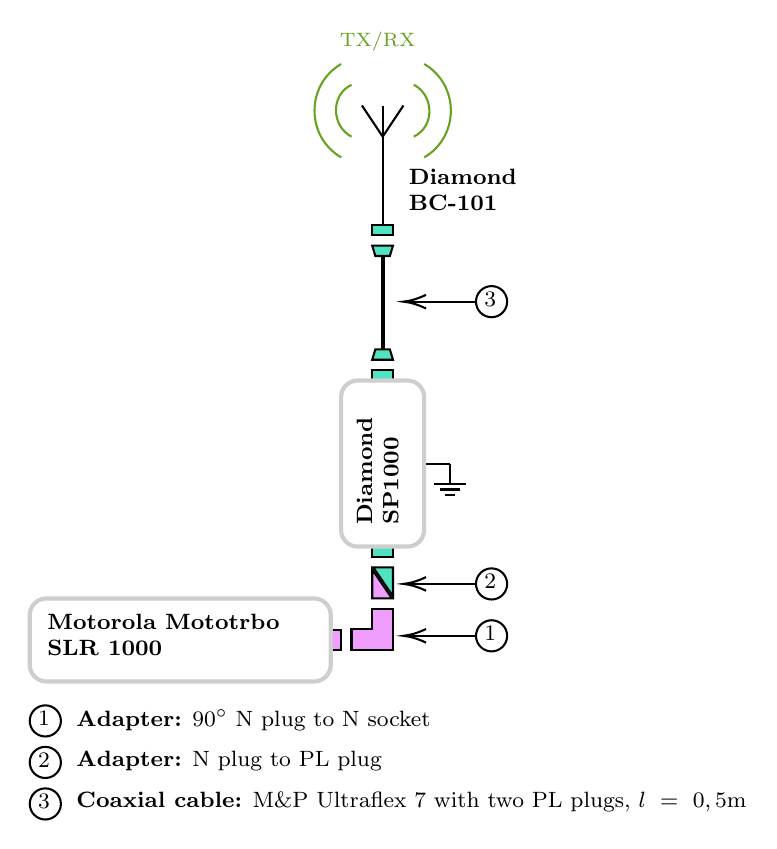
\begin{tikzpicture}[x=0.75pt,y=0.75pt,yscale=-1,xscale=1]
%uncomment if require: \path (0,463); %set diagram left start at 0, and has height of 463

%Straight Lines [id:da2117409366899652] 
\draw    (345,270) -- (357.5,270) ;
%Straight Lines [id:da19758281728068594] 
\draw    (357.5,270) -- (357.5,280) ;
%Straight Lines [id:da9706348152903634] 
\draw    (350,280) -- (365,280) ;
%Straight Lines [id:da9955066685628202] 
\draw    (352.5,282.5) -- (362.5,282.5) ;
%Straight Lines [id:da3542838525324348] 
\draw    (355,285) -- (360,285) ;

%Shape: Rectangle [id:dp5195215226134675] 
\draw  [fill={rgb, 255:red, 80; green, 227; blue, 194 }  ,fill opacity=1 ] (320,230) -- (320,225) -- (330,225) -- (330,230) -- cycle ;
%Shape: Rectangle [id:dp04379129192102571] 
\draw  [fill={rgb, 255:red, 80; green, 227; blue, 194 }  ,fill opacity=1 ] (320,315) -- (320,310) -- (330,310) -- (330,315) -- cycle ;
%Rounded Rect [id:dp609897861214854] 
\draw  [color={rgb, 255:red, 206; green, 206; blue, 206 }  ,draw opacity=1 ][line width=1.5]  (313,310) .. controls (308.58,310) and (305,306.42) .. (305,302) -- (305,238) .. controls (305,233.58) and (308.58,230) .. (313,230) -- (337,230) .. controls (341.42,230) and (345,233.58) .. (345,238) -- (345,302) .. controls (345,306.42) and (341.42,310) .. (337,310) -- cycle ;


%Straight Lines [id:da8216628264555428] 
\draw    (325.04,97.5) -- (325.04,157.5) ;
%Straight Lines [id:da11975977315738118] 
\draw    (315.04,97.5) -- (325.04,112.5) ;
%Straight Lines [id:da2623857929633875] 
\draw    (325.04,112.5) -- (335.04,97.5) ;
%Curve Lines [id:da9838947299311864] 
\draw [color={rgb, 255:red, 101; green, 162; blue, 30 }  ,draw opacity=1 ]   (340.04,87.5) .. controls (349.76,92.5) and (350.33,107.64) .. (340.04,112.5) ;
%Curve Lines [id:da48333252009100747] 
\draw [color={rgb, 255:red, 101; green, 162; blue, 30 }  ,draw opacity=1 ]   (345.04,77.5) .. controls (362.29,87.63) and (362.04,112.63) .. (345.04,122.5) ;

%Curve Lines [id:da06276736990916465] 
\draw [color={rgb, 255:red, 101; green, 162; blue, 30 }  ,draw opacity=1 ]   (310.04,112.5) .. controls (300.33,107.5) and (299.76,92.36) .. (310.04,87.5) ;
%Curve Lines [id:da8544747440552438] 
\draw [color={rgb, 255:red, 101; green, 162; blue, 30 }  ,draw opacity=1 ]   (305.04,122.5) .. controls (287.79,112.38) and (288.04,87.37) .. (305.04,77.5) ;

%Shape: Rectangle [id:dp5540086456806208] 
\draw  [fill={rgb, 255:red, 80; green, 227; blue, 194 }  ,fill opacity=1 ] (320.04,155) -- (330.04,155) -- (330.04,160) -- (320.04,160) -- cycle ;
%Shape: Rectangle [id:dp17515633991893775] 
\draw  [fill={rgb, 255:red, 239; green, 158; blue, 255 }  ,fill opacity=1 ] (300,350) -- (305,350) -- (305,360) -- (300,360) -- cycle ;
%Rounded Rect [id:dp7223835974557309] 
\draw  [color={rgb, 255:red, 206; green, 206; blue, 206 }  ,draw opacity=1 ][line width=1.5]  (155,343) .. controls (155,338.58) and (158.58,335) .. (163,335) -- (292,335) .. controls (296.42,335) and (300,338.58) .. (300,343) -- (300,367) .. controls (300,371.42) and (296.42,375) .. (292,375) -- (163,375) .. controls (158.58,375) and (155,371.42) .. (155,367) -- cycle ;


%Shape: Path Data [id:dp2172730430252452] 
\draw  [fill={rgb, 255:red, 239; green, 158; blue, 255 }  ,fill opacity=1 ] (310,360) -- (310,349.67) -- (320,349.67) -- (320,340) -- (330,340) -- (330,360) -- (310,360) -- cycle ;
%Shape: Right Triangle [id:dp30746565461403486] 
\draw  [fill={rgb, 255:red, 80; green, 227; blue, 194 }  ,fill opacity=1 ] (320.48,320) -- (330,333.98) -- (330,320) -- cycle ;
%Shape: Right Triangle [id:dp7515173690048442] 
\draw  [fill={rgb, 255:red, 239; green, 158; blue, 255 }  ,fill opacity=1 ] (329.52,335) -- (320,321.02) -- (320,335) -- cycle ;

%Straight Lines [id:da9120395561613033] 
\draw [line width=1.5]    (325,170) -- (325,215) ;
%Shape: Trapezoid [id:dp9006012786033941] 
\draw  [fill={rgb, 255:red, 80; green, 227; blue, 194 }  ,fill opacity=1 ][line width=0.75]  (330,165) -- (328.5,170) -- (321.5,170) -- (320,165) -- cycle ;
%Shape: Trapezoid [id:dp20960810518276118] 
\draw  [fill={rgb, 255:red, 80; green, 227; blue, 194 }  ,fill opacity=1 ][line width=0.75]  (320,220) -- (321.5,215) -- (328.5,215) -- (330,220) -- cycle ;

%Straight Lines [id:da35692414312633214] 
\draw    (370,353) -- (337,353) ;
\draw [shift={(335,353)}, rotate = 360] [color={rgb, 255:red, 0; green, 0; blue, 0 }  ][line width=0.75]    (10.93,-3.29) .. controls (6.95,-1.4) and (3.31,-0.3) .. (0,0) .. controls (3.31,0.3) and (6.95,1.4) .. (10.93,3.29)   ;
%Shape: Circle [id:dp44275798239943964] 
\draw   (370,353) .. controls (370,348.86) and (373.36,345.5) .. (377.5,345.5) .. controls (381.64,345.5) and (385,348.86) .. (385,353) .. controls (385,357.14) and (381.64,360.5) .. (377.5,360.5) .. controls (373.36,360.5) and (370,357.14) .. (370,353) -- cycle ;


%Shape: Circle [id:dp08416294362563437] 
\draw   (370,328) .. controls (370,323.86) and (373.36,320.5) .. (377.5,320.5) .. controls (381.64,320.5) and (385,323.86) .. (385,328) .. controls (385,332.14) and (381.64,335.5) .. (377.5,335.5) .. controls (373.36,335.5) and (370,332.14) .. (370,328) -- cycle ;

%Straight Lines [id:da011949664490807699] 
\draw    (370,328) -- (337,328) ;
\draw [shift={(335,328)}, rotate = 360] [color={rgb, 255:red, 0; green, 0; blue, 0 }  ][line width=0.75]    (10.93,-3.29) .. controls (6.95,-1.4) and (3.31,-0.3) .. (0,0) .. controls (3.31,0.3) and (6.95,1.4) .. (10.93,3.29)   ;

%Shape: Circle [id:dp29561759695484313] 
\draw   (370,192) .. controls (370,187.86) and (373.36,184.5) .. (377.5,184.5) .. controls (381.64,184.5) and (385,187.86) .. (385,192) .. controls (385,196.14) and (381.64,199.5) .. (377.5,199.5) .. controls (373.36,199.5) and (370,196.14) .. (370,192) -- cycle ;

%Straight Lines [id:da6708191132816714] 
\draw    (370,192) -- (337,192) ;
\draw [shift={(335,192)}, rotate = 360] [color={rgb, 255:red, 0; green, 0; blue, 0 }  ][line width=0.75]    (10.93,-3.29) .. controls (6.95,-1.4) and (3.31,-0.3) .. (0,0) .. controls (3.31,0.3) and (6.95,1.4) .. (10.93,3.29)   ;

%Shape: Circle [id:dp6925244802161248] 
\draw   (155,394) .. controls (155,389.86) and (158.36,386.5) .. (162.5,386.5) .. controls (166.64,386.5) and (170,389.86) .. (170,394) .. controls (170,398.14) and (166.64,401.5) .. (162.5,401.5) .. controls (158.36,401.5) and (155,398.14) .. (155,394) -- cycle ;

%Shape: Circle [id:dp5144865887931986] 
\draw   (155,414) .. controls (155,409.86) and (158.36,406.5) .. (162.5,406.5) .. controls (166.64,406.5) and (170,409.86) .. (170,414) .. controls (170,418.14) and (166.64,421.5) .. (162.5,421.5) .. controls (158.36,421.5) and (155,418.14) .. (155,414) -- cycle ;

%Shape: Circle [id:dp2881120818061964] 
\draw   (155,434) .. controls (155,429.86) and (158.36,426.5) .. (162.5,426.5) .. controls (166.64,426.5) and (170,429.86) .. (170,434) .. controls (170,438.14) and (166.64,441.5) .. (162.5,441.5) .. controls (158.36,441.5) and (155,438.14) .. (155,434) -- cycle ;



% Text Node
\draw (157.5,428) node [anchor=north west][inner sep=0.75pt]  [font=\footnotesize] [align=left] {3};
% Text Node
\draw (157.5,408) node [anchor=north west][inner sep=0.75pt]  [font=\footnotesize] [align=left] {2};
% Text Node
\draw (157.5,388) node [anchor=north west][inner sep=0.75pt]  [font=\footnotesize] [align=left] {1};
% Text Node
\draw (372.5,186) node [anchor=north west][inner sep=0.75pt]  [font=\footnotesize] [align=left] {3};
% Text Node
\draw (372.5,322) node [anchor=north west][inner sep=0.75pt]  [font=\footnotesize] [align=left] {2};
% Text Node
\draw (372.5,347) node [anchor=north west][inner sep=0.75pt]  [font=\footnotesize] [align=left] {1};
% Text Node
\draw (302.89,60.5) node [anchor=north west][inner sep=0.75pt]  [font=\scriptsize,color={rgb, 255:red, 101; green, 162; blue, 30 }  ,opacity=1 ] [align=left] {TX/RX};
% Text Node
\draw (311,301) node [anchor=north west][inner sep=0.75pt]  [font=\footnotesize,rotate=-270] [align=left] {\textbf{Diamond}\\\textbf{SP1000}};
% Text Node
\draw (162,341) node [anchor=north west][inner sep=0.75pt]  [font=\footnotesize] [align=left] {\textbf{Motorola Mototrbo}\\\textbf{SLR 1000}};
% Text Node
\draw (336.2,126.5) node [anchor=north west][inner sep=0.75pt]  [font=\footnotesize] [align=left] {\textbf{Diamond }\\\textbf{BC-101}};
% Text Node
\draw (176,427) node [anchor=north west][inner sep=0.75pt]  [font=\footnotesize] [align=left] {\textbf{Coaxial cable:} M\&P Ultraflex 7 with two PL plugs, $\displaystyle l\ =\ 0,5\mathrm{m}$};
% Text Node
\draw (176,407) node [anchor=north west][inner sep=0.75pt]  [font=\footnotesize] [align=left] {\textbf{Adapter:} N plug to PL plug};
% Text Node
\draw (176,387) node [anchor=north west][inner sep=0.75pt]  [font=\footnotesize] [align=left] {\textbf{Adapter:} $\displaystyle 90^{\circ }$ N plug to N socket};


\end{tikzpicture}

	\caption{Schematic structure of repeater radio infrastructure.}
	\label{fig:tikz_repeater}
\end{figure}

Using the specifications of the SLR 1000 listed in the table \ref{tab:table_slr1000_specs}, the maximum transmission power is calculated in the equation (\ref{eq:power_rep_tx}). The minimum required reception power for the worst case can be taken from the equation (\ref{eq:power_BSt_min}).
\begin{table}[h!] % SLR1000
	\centering
	\footnotesize
\begin{tabular}{|l|c|}
	\hline
	\multicolumn{2}{|c|}{\textbf{Motorola Mototrbo SLR 1000 (VHF digital) specifications}} \\
	\hline
 	Frequency & $136\mathrm{MHz}$ to $174\mathrm{MHz}$ \\
	System impedance & $50\Omega$\\
 	Dimensions $\mathrm{(H \times W \times D)}$ & $279 \times 229 \times 102 \mathrm{mm}$ \\%
 	Mass & $4,54\mathrm{kg}$ \\%
	Power supply & $12\mathrm{VDC}$ ($11,0$ to $15,5\mathrm{VDC}$) \\
	Current RX and standby & $0,7\mathrm{A}$ ($0,63\mathrm{A}$ typical) \\
	Current TX & $3\mathrm{A}$ (max.) \\
	Operating temperature & $-30^\circ \mathrm{C}$ to $60^\circ \mathrm{C}$ \\
	RX sensitivity 5\% BER: & $0,25\mathrm{\mu V}$ ($0,18\mathrm{\mu V}$ typical) \\
	TX power output & $1\mathrm{W}$ to $10\mathrm{W}$ \\
	Connector & N socket\\
	IP rating & $65$\\
	\hline
\end{tabular}
	\caption{Excerpt from the data sheet of the Motorola Mototrbo SLR 1000 repeater. \cite{SLR1000:2019}}
	\label{tab:table_slr1000_specs}
\end{table}
\begin{equation} \label{eq:power_rep_tx}
	\centering
	P_\mathrm{T,dBW} =  10\mathrm{dBW} \cdot \log_{10} \left( \dfrac{10\mathrm{W}}{1\mathrm{W}} \right) = 10\mathrm{dBW}\text{,}
\end{equation}

Since the repeater uses the same lightning arrester and the same antenna as the base station, the resulting losses can be taken directly from the equations (\ref{eq:losses_BSt_arr}) and (\ref{eq:losses_BSt_ant}). The antenna of the repeater is always mounted at a height of $h_\mathrm{REP} = 8\mathrm{m}$ above the ground, as a mast is included in the system design. 

As can be seen in the figure \ref{fig:tikz_repeater}, the length of the coaxial cable is $0,5\mathrm{m}$, resulting in an insertion loss of:   
\begin{equation} \label{eq:losses_BSt_coax}
	\centering
	L_\mathrm{coax,dB} = \dfrac{7,2471 \cdot 0,5}{100}\mathrm{dB} = 0,036\mathrm{dB}\text{.}
\end{equation}

With the number of adapters and connectors $N_\mathrm{I} = 4$, their insertion loss follows to:
\begin{equation} \label{eq:losses_rep_conn}
	\centering
	L_\mathrm{conn/adapt,dB} = 0,4\mathrm{dB}\text{.}
\end{equation}

Finally, the total loss of the antenna feed line can be calculated with:
\begin{equation} \label{eq:losses_rep}
	\centering
	L_\mathrm{REP,dB} = L_\mathrm{arr,dB} + L_\mathrm{ant,dB} + L_\mathrm{coax,dB} + L_\mathrm{conn/adapt,dB} = 0,849\mathrm{dB}\text{.}
\end{equation}

\subsection{Serenity radio system}
As mentioned earlier, Serenity is the spacesuit simulator that the AAs use to conduct analog Mars missions. Its radio system consists of a Motorola Mototrbo SL 2600 handheld radio with a Motorola PMAD4156A antenna, a \emph{push-to-talk} (PTT) button and a Jabra Storm Bluetooth headset. The antenna is attached directly to the handheld radio and the entire system is built into the spacesuit simulator with the upper part of the antenna sticking out. Since the SL 2600 radio supports Bluetooth 4.0, it was decided that communication with the headset should take place via Bluetooth. This has two advantages. Firstly, the AA can put on the headset before donning and thus simply step into the spacesuit simulator, and secondly, the amount of cabling is reduced. The PTT button is wired to the outside of the spacesuit so that the AA can press it to communicate. A schematic structure of this system is illustrated in the figure \ref{fig:tikz_serenity_radio_system}.
\begin{figure}[h!]
	\centering
	

\tikzset{every picture/.style={line width=0.75pt}} %set default line width to 0.75pt        

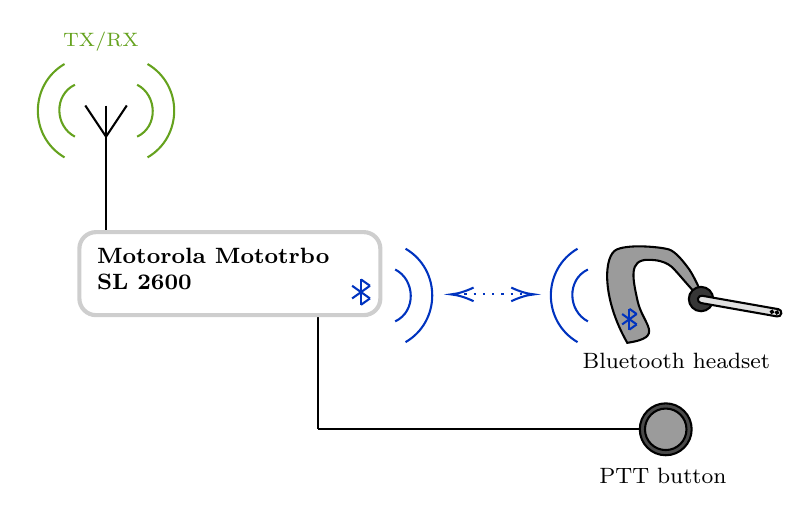
\begin{tikzpicture}[x=0.75pt,y=0.75pt,yscale=-1,xscale=1]
%uncomment if require: \path (0,611); %set diagram left start at 0, and has height of 611

%Straight Lines [id:da6025377414505892] 
\draw    (275,365) -- (275,420) ;
%Straight Lines [id:da8632563010362544] 
\draw    (172.84,264) -- (172.84,324) ;
%Straight Lines [id:da9125480475574657] 
\draw    (162.84,264) -- (172.84,279) ;
%Straight Lines [id:da061481860873287] 
\draw    (172.84,279) -- (182.84,264) ;
%Curve Lines [id:da709923124702297] 
\draw [color={rgb, 255:red, 101; green, 162; blue, 30 }  ,draw opacity=1 ]   (187.84,254) .. controls (197.56,259) and (198.13,274.14) .. (187.84,279) ;
%Curve Lines [id:da449825910233995] 
\draw [color={rgb, 255:red, 101; green, 162; blue, 30 }  ,draw opacity=1 ]   (192.84,244) .. controls (210.09,254.13) and (209.84,279.13) .. (192.84,289) ;

%Curve Lines [id:da6587381411545086] 
\draw [color={rgb, 255:red, 101; green, 162; blue, 30 }  ,draw opacity=1 ]   (157.84,279) .. controls (148.13,274) and (147.56,258.86) .. (157.84,254) ;
%Curve Lines [id:da5450398860583288] 
\draw [color={rgb, 255:red, 101; green, 162; blue, 30 }  ,draw opacity=1 ]   (152.84,289) .. controls (135.59,278.88) and (135.84,253.87) .. (152.84,244) ;

%Rounded Rect [id:dp4917700194036718] 
\draw  [color={rgb, 255:red, 206; green, 206; blue, 206 }  ,draw opacity=1 ][line width=1.5]  (160,333) .. controls (160,328.58) and (163.58,325) .. (168,325) -- (297,325) .. controls (301.42,325) and (305,328.58) .. (305,333) -- (305,357) .. controls (305,361.42) and (301.42,365) .. (297,365) -- (168,365) .. controls (163.58,365) and (160,361.42) .. (160,357) -- cycle ;

%Straight Lines [id:da4309100693896566] 
\draw [color={rgb, 255:red, 0; green, 51; blue, 191 }  ,draw opacity=1 ]   (291.4,350.85) -- (300,356.95) ;
%Straight Lines [id:da87178799188694] 
\draw [color={rgb, 255:red, 0; green, 51; blue, 191 }  ,draw opacity=1 ]   (291.4,356.95) -- (300,350.85) ;
%Straight Lines [id:da19897395538792528] 
\draw [color={rgb, 255:red, 0; green, 51; blue, 191 }  ,draw opacity=1 ]   (295.7,360) -- (295.7,347.8) ;
%Straight Lines [id:da6954421251039244] 
\draw [color={rgb, 255:red, 0; green, 51; blue, 191 }  ,draw opacity=1 ]   (295.7,347.8) -- (300,350.85) ;
%Straight Lines [id:da6576758812784198] 
\draw [color={rgb, 255:red, 0; green, 51; blue, 191 }  ,draw opacity=1 ]   (300,356.95) -- (295.7,360) ;

%Curve Lines [id:da8176024686496981] 
\draw [color={rgb, 255:red, 0; green, 51; blue, 191 }  ,draw opacity=1 ]   (312.16,343) .. controls (321.87,348) and (322.44,363.14) .. (312.16,368) ;
%Curve Lines [id:da5314914665000634] 
\draw [color={rgb, 255:red, 0; green, 51; blue, 191 }  ,draw opacity=1 ]   (317.16,333) .. controls (334.41,343.13) and (334.16,368.13) .. (317.16,378) ;

%Straight Lines [id:da8982122185779959] 
\draw    (275,420) -- (430,420) ;
%Shape: Circle [id:dp17058876030974823] 
\draw  [fill={rgb, 255:red, 74; green, 74; blue, 74 }  ,fill opacity=1 ] (430,420) .. controls (430,413.1) and (435.6,407.5) .. (442.5,407.5) .. controls (449.4,407.5) and (455,413.1) .. (455,420) .. controls (455,426.9) and (449.4,432.5) .. (442.5,432.5) .. controls (435.6,432.5) and (430,426.9) .. (430,420) -- cycle ;
%Shape: Circle [id:dp8498841036551381] 
\draw  [fill={rgb, 255:red, 155; green, 155; blue, 155 }  ,fill opacity=1 ] (432.5,420) .. controls (432.5,414.48) and (436.98,410) .. (442.5,410) .. controls (448.02,410) and (452.5,414.48) .. (452.5,420) .. controls (452.5,425.52) and (448.02,430) .. (442.5,430) .. controls (436.98,430) and (432.5,425.52) .. (432.5,420) -- cycle ;
%Curve Lines [id:da06702286308124483] 
\draw [color={rgb, 255:red, 0; green, 51; blue, 191 }  ,draw opacity=1 ]   (405,368) .. controls (395.29,363) and (394.71,347.86) .. (405,343) ;
%Curve Lines [id:da6829496922473743] 
\draw [color={rgb, 255:red, 0; green, 51; blue, 191 }  ,draw opacity=1 ]   (400,378) .. controls (382.75,367.88) and (383,342.88) .. (400,333) ;

%Curve Lines [id:da5138620347394718] 
\draw [fill={rgb, 255:red, 155; green, 155; blue, 155 }  ,fill opacity=1 ]   (423.98,378.33) .. controls (411.48,356.58) and (412.48,336.08) .. (418.98,333.33) .. controls (425.48,330.58) and (440.82,332.33) .. (443.98,333.33) .. controls (447.14,334.33) and (450.67,338.7) .. (453.5,342.52) .. controls (456.33,346.33) and (462.98,360.59) .. (459.5,357.24) .. controls (456.02,353.89) and (449.86,346.52) .. (447.86,344.33) .. controls (445.86,342.15) and (443.32,338.33) .. (433.98,338.33) .. controls (424.64,338.33) and (426.48,347.08) .. (428.98,358.33) .. controls (431.48,369.58) and (442.48,375.58) .. (423.98,378.33) -- cycle ;
%Shape: Circle [id:dp8048282894012855] 
\draw  [fill={rgb, 255:red, 54; green, 54; blue, 54 }  ,fill opacity=1 ] (453.63,357.24) .. controls (453.63,354) and (456.26,351.37) .. (459.5,351.37) .. controls (462.74,351.37) and (465.38,354) .. (465.38,357.24) .. controls (465.38,360.49) and (462.74,363.12) .. (459.5,363.12) .. controls (456.26,363.12) and (453.63,360.49) .. (453.63,357.24) -- cycle ;
%Rounded Rect [id:dp33219306299895135] 
\draw  [fill={rgb, 255:red, 225; green, 225; blue, 225 }  ,fill opacity=1 ] (458.01,357.1) .. controls (458.18,356.14) and (459.11,355.49) .. (460.07,355.66) -- (496.75,362.12) .. controls (497.72,362.29) and (498.36,363.21) .. (498.19,364.18) -- (498.19,364.18) .. controls (498.02,365.15) and (497.1,365.8) .. (496.13,365.62) -- (459.46,359.16) .. controls (458.49,358.99) and (457.84,358.07) .. (458.01,357.1) -- cycle ;
%Shape: Circle [id:dp48821144483641965] 
\draw   (495.61,363.62) .. controls (495.68,363.35) and (495.95,363.19) .. (496.22,363.26) .. controls (496.49,363.33) and (496.65,363.61) .. (496.58,363.87) .. controls (496.51,364.14) and (496.23,364.3) .. (495.97,364.23) .. controls (495.7,364.16) and (495.54,363.89) .. (495.61,363.62) -- cycle ;
%Shape: Circle [id:dp10261371159326838] 
\draw   (493.19,363.28) .. controls (493.26,363.01) and (493.53,362.85) .. (493.8,362.92) .. controls (494.07,362.99) and (494.23,363.26) .. (494.16,363.53) .. controls (494.09,363.8) and (493.81,363.96) .. (493.55,363.89) .. controls (493.28,363.82) and (493.12,363.54) .. (493.19,363.28) -- cycle ;

%Straight Lines [id:da7564970333053862] 
\draw [color={rgb, 255:red, 0; green, 51; blue, 191 }  ,draw opacity=1 ]   (421.5,364.46) -- (428.5,369.46) ;
%Straight Lines [id:da16147426128772913] 
\draw [color={rgb, 255:red, 0; green, 51; blue, 191 }  ,draw opacity=1 ]   (421.5,369.46) -- (428.5,364.46) ;
%Straight Lines [id:da9003409214844904] 
\draw [color={rgb, 255:red, 0; green, 51; blue, 191 }  ,draw opacity=1 ]   (425,371.96) -- (425,361.96) ;
%Straight Lines [id:da47263261295445824] 
\draw [color={rgb, 255:red, 0; green, 51; blue, 191 }  ,draw opacity=1 ]   (425,361.96) -- (428.5,364.46) ;
%Straight Lines [id:da30877576094905756] 
\draw [color={rgb, 255:red, 0; green, 51; blue, 191 }  ,draw opacity=1 ]   (428.5,369.46) -- (425,371.96) ;

%Straight Lines [id:da6981946954878862] 
\draw [color={rgb, 255:red, 0; green, 51; blue, 191 }  ,draw opacity=1 ] [dash pattern={on 0.84pt off 2.51pt}]  (341,355) -- (377,355) ;
\draw [shift={(379,355)}, rotate = 180] [color={rgb, 255:red, 0; green, 51; blue, 191 }  ,draw opacity=1 ][line width=0.75]    (10.93,-3.29) .. controls (6.95,-1.4) and (3.31,-0.3) .. (0,0) .. controls (3.31,0.3) and (6.95,1.4) .. (10.93,3.29)   ;
\draw [shift={(339,355)}, rotate = 0] [color={rgb, 255:red, 0; green, 51; blue, 191 }  ,draw opacity=1 ][line width=0.75]    (10.93,-3.29) .. controls (6.95,-1.4) and (3.31,-0.3) .. (0,0) .. controls (3.31,0.3) and (6.95,1.4) .. (10.93,3.29)   ;

% Text Node
\draw (167,331) node [anchor=north west][inner sep=0.75pt]  [font=\footnotesize] [align=left] {\textbf{Motorola Mototrbo}\\\textbf{SL 2600}};
% Text Node
\draw (150.69,227) node [anchor=north west][inner sep=0.75pt]  [font=\scriptsize,color={rgb, 255:red, 101; green, 162; blue, 30 }  ,opacity=1 ] [align=left] {TX/RX};
% Text Node
\draw (401,382) node [anchor=north west][inner sep=0.75pt]  [font=\footnotesize] [align=left] {Bluetooth headset};
% Text Node
\draw (409,437) node [anchor=north west][inner sep=0.75pt]  [font=\footnotesize] [align=left] {PTT button};


\end{tikzpicture}

	\caption{Schematic structure of the Serenity radio system.}
	\label{fig:tikz_serenity_radio_system}
\end{figure}

Electrical energy is provided to the SL 2600 via its $2,3\mathrm{Ah}$ lithium-ion battery (Motorola PMNN4468B) which is charged with the electrical energy from the local power grid between missions. At a later point in time, the radio system can be upgraded in such a way, that the SL 2600 can be directly charged from the spacesuit simulator. Similar to the SL 2600, the Bluetooth headset is also supplied with electrical energy from its battery, but can only be charged via the local power grid. 

The maximum transmission power of the SL 2600, as shown in the equation (\ref{eq:power_SER_tx}), is calculated based on its specifications in the table \ref{tab:table_sl2600_specs}.
\begin{table}[h!] % SL2600
	\centering
	\footnotesize
\begin{tabular}{|l|c|}
	\hline
	\multicolumn{2}{|c|}{\textbf{Motorola Mototrbo SL 2600 (VHF digital) specifications}} \\
	\hline
 	Frequency & $136\mathrm{MHz}$ to $174\mathrm{MHz}$ \\
 	Dimensions $\mathrm{(H \times W \times D)}$ & $125,7 \times 55,0 \times 22,7 \mathrm{mm}$ \\%
 	Mass (incl. std. battery) & $190\mathrm{g}$ \\%
	Power supply & $3,7\mathrm{VDC}$ (nominal) \\
 	Average battery life at 5/5/90 duty cycle & $13,5\mathrm{h}$ \\
	Operating temperature & $-30^\circ \mathrm{C}$ to $60^\circ \mathrm{C}$ \\
	Storage temperature & $-40^\circ \mathrm{C}$ to $85^\circ \mathrm{C}$ \\
	RX sensitivity 5\% BER: & $0,25\mathrm{\mu V}$ ($0,19\mathrm{\mu V}$ typical) \\
	TX power output & $0,5\mathrm{W}$ to $3\mathrm{W}$ \\
	Bluetooth version & $4,0$\\
	IP rating & $54$\\
	\hline
\end{tabular}
	\caption{Excerpt from the data sheet of the Motorola Mototrbo SL 2600 handheld radio. \cite{SL2600:2017}}
	\label{tab:table_sl2600_specs}
\end{table}
\begin{equation} \label{eq:power_SER_tx}
	\centering
	P_\mathrm{T,dBW} =  10\mathrm{dBW} \cdot \log_{10} \left( \dfrac{3\mathrm{W}}{1\mathrm{W}} \right) = 4,771\mathrm{dBW}\text{,}
\end{equation}
As with the SLR 1000, the minimum required reception power for the worst case can be taken from the equation (\ref{eq:power_BSt_min}). At this point, the assumption is made that the antenna impedance is $50\Omega$, as no further specifications could be found. It was furthermore assumed that there are no losses in the antenna feed line and that the antenna has a gain of $0\mathrm{dBi}$. 


In cooperation with the Serenity \emph{structures} (STRUC) team, a position for the SL 2600 in the HUT of the spacesuit simulator was found, so that its antenna is upright at a height of $1,65\mathrm{m}$ above the ground for a standard male AA, or at a height of $1,55\mathrm{m}$ above the ground for a standard female AA \cite{Hinker:2007}. Regarding the link budget estimation $h_\mathrm{SER} = 1,55\mathrm{m}$ is used. In its installed position the device can be recharged and, if necessary, removed for maintenance purposes. This fulfills the requirement that the Serenity radio system must fit into the HUT. 

Taking into account the requirements for the operating temperature of the radio system, the data sheets of the SL 2600 (see table \ref{tab:table_sl2600_specs}) and the PTT button, including the wires and connectors involved, show that these are met. Due to the large push area of the PTT button, it was adopted from the Aouda spacesuit simulator, which is the predecessor of Serenity. No specifications were found for the Bluetooth headset and the audio jack that connects the PTT button to the SL 2600. The prototype still needs to be tested in this regard. However, if these do not meet the requirements, a suitable audio jack can be requested directly from Motorola Solutions Inc. and the Motorola EP900w Bluetooth headset can be procured \cite{push_switch:2011, EP900w:2021}.

The most important factor that needed to be considered when developing the radio system was its mass. As stated in the requirements, the combined mass of the W-LAN and VHF based communication systems must not exceed $1000\mathrm{g}$. At the time the Serenity (VHF) radio system was developed, the W-LAN based communication system had a mass of $605,33\mathrm{g}$. The total mass of the (VHF) radio system is $248\mathrm{g}$. This results in a combined mass of $853,33\mathrm{g}$. $9\mathrm{g}$ of this is the mass of the Jabra Storm Bluetooth headset. Should it be replaced by the Motorola EP900w Bluetooth headset, the (VHF) radio system would then have a mass of $261\mathrm{g}$, which results in a combined mass of $866,33\mathrm{g}$. The measurements were conducted with a digital kitchen scale from WMF (Model No.: 06.0873.6040). In the case that the audio jack needs to be changed, its mass is likely to remain the same. Since the W-LAN based communication system is not finished, it cannot be said at this point whether the mass requirement has
 been met. 


\subsection{Safety officer radio}
The safety officers do not interact directly with the AAs during an ongoing mission, but intervene in certain events. During these events it is crucial that voice communication is established between these two groups. For this purpose, the safety officers use a Motorola Mototrbo SL 2600 handheld radio with the same antenna and lithium-ion battery as that of the AAs. The battery of the SL 2600 is charged by the local power grid between missions.

The maximum transmission power is the same as in the equation (\ref{eq:power_SER_tx}) and the minimum required reception power for the worst case is the same as in the equation (\ref{eq:power_BSt_min}).

Regarding the antenna, the same assumptions are made as for the Serenity radio system. However, its height above the ground was determined based on the anthropometric dimensional data for an american female and male, shown in the figures \ref{fig:image_female} and \ref{fig:image_male}.
\begin{figure}[h!]
	\centering
	\begin{subfigure}[b]{0.3\textwidth}
		\centering
		\includegraphics[width = \textwidth]{image_female}
		\caption{\textit{``Body Size of the 40-Year-Old Japanese Female for Year 2000 in One Gravity Conditions.''} \textbf{23} $\widehat{=}$ 1,271m.}
		\label{fig:image_female}
	\end{subfigure}
	\hspace{60pt}
	\begin{subfigure}[b]{0.3\textwidth}
		\centering
		\includegraphics[width = \textwidth]{image_male}
		\caption{\textit{``Body Size of the 40-Year-Old American Male for Year 2000 in One Gravity Conditions.''} \textbf{23} $\widehat{=}$ 1,476m.}
		\label{fig:image_male}
	\end{subfigure}
	\caption{Anthropometric dimensional data for the american female and male. (Image and caption credit: \cite{Hinker:2007, Adolf:2020})}
	\label{fig:bodies}
\end{figure}
When it is assumed that the SL 2600 is operated at shoulder height, then its antenna is $1,271\mathrm{m}$ above the ground for a female and $1,476\mathrm{m}$ above the ground for a male safety officer \cite{Hinker:2007, Adolf:2020}. For the link budget estimation $h_\mathrm{SFTY} = 1,271\mathrm{m}$ is used.
\subsection{On-site support crew radio}
The on-site support crew, which carries out general tasks in the mission area, uses the DP 3601 handheld radios. These are supplied with electrical energy from their $2,15\mathrm{Ah}$ lithium-ion batteries (Motorola PMNN4103A) which are charged via the local power grid when required.  

According to the same principle as in the previous subsections, the maximum transmission power of the DP 3601 can be calculated using the equation (\ref{eq:power_OSS_tx}), with its specifications being listed in the table \ref{tab:table_dp3601_specs}.
\begin{table}[h!] % DP3601
	\centering
	\footnotesize
\begin{tabular}{|l|c|}
	\hline
	\multicolumn{2}{|c|}{\textbf{Motorola Mototrbo DP 3601 (VHF digital) specifications}} \\
	\hline
 	Frequency & $136\mathrm{MHz}$ to $174\mathrm{MHz}$ \\
 	Dimensions $\mathrm{(H \times W \times D)}$ & $131,5 \times 63,5 \times 35,2 \mathrm{mm}$ \\%
 	Mass (incl. $2200\mathrm{mAh}$ li-ion battery) & $361\mathrm{g}$ \\%
	Power supply & $7,5\mathrm{VDC}$ (nominal) \\
 	Average battery life at 5/5/90 duty cycle & $19,0\mathrm{h}$ \\
	Operating temperature & $-30^\circ \mathrm{C}$ to $60^\circ \mathrm{C}$ \\
	Storage temperature & $-40^\circ \mathrm{C}$ to $85^\circ \mathrm{C}$ \\
	RX sensitivity 5\% BER: & $0,30\mathrm{\mu V}$ \\
	TX power output & $1\mathrm{W}$ to $5\mathrm{W}$ \\
	IP rating & $57$\\
	\hline
\end{tabular}
	\caption{Excerpt from the data sheet of the Motorola Mototrbo DP 3601 handheld radio. \cite{DP3601:2010}}
	\label{tab:table_dp3601_specs}
\end{table}
\begin{equation} \label{eq:power_OSS_tx}
	\centering
	P_\mathrm{T,dBW} =  10\mathrm{dBW} \cdot \log_{10} \left( \dfrac{5\mathrm{W}}{1\mathrm{W}} \right) = 6,99\mathrm{dBW}\text{,}
\end{equation}
Since the DP 3601 is an older handheld radio, its sensitivity differs from that of the other Motorola Mototrbo radio devices mentioned earlier. By assuming that the antenna impedance is $50\Omega$ -- due to the same reasons as for the SL 2600 -- the minimum required reception power follows to:
\begin{equation} \label{eq:power_OSS_min}
	\centering
	P_\mathrm{min,dBW} = 10\mathrm{dBW} \cdot \log_{10} \left( \dfrac{\left(0,30\cdot10^{-6}\mathrm{V}\right)^2}{50\Omega} \right) = -147,447\mathrm{dBW}\text{.}
\end{equation}

The antenna of the DP 3601 is directly attached to the radio and it is assumed, that no losses in the antenna feed line occur. Furthermore, its gain is assumed to be $0\mathrm{dBi}$ and, as in the previous subsection, its hight above the ground is assumed to be $h_\mathrm{OSS} = 1,271\mathrm{m}$.





